% \iffalse meta-comment
%
% Copyright (C) 2017--2020 by Xiangdong Zeng <xdzeng96@gmail.com>
%
% This work may be distributed and/or modified under the
% conditions of the LaTeX Project Public License, either
% version 1.3c of this license or (at your option) any later
% version. The latest version of this license is in:
%
%   http://www.latex-project.org/lppl.txt
%
% and version 1.3 or later is part of all distributions of
% LaTeX version 2005/12/01 or later.
%
% This work has the LPPL maintenance status `maintained'.
%
% The Current Maintainer of this work is Xiangdong Zeng.
%
% \fi

%*********************************************************************
% fduthesis: 复旦大学论文模板
% 2020/08/30 v0.7e
%
% 重要提示:
%   1. 请确保使用 UTF-8 编码保存
%   2. 请使用 XeLaTeX 或 LuaLaTeX 编译
%   3. 请仔细阅读用户文档
%   4. 修改、使用、发布本文档请务必遵循 LaTeX Project Public License
%   5. 不需要的注释可以尽情删除
%*********************************************************************

\documentclass[type=master,oneside]{fduthesis}
% 模板选项:
%   type = doctor|master|bachelor  论文类型,默认为本科论文
%   oneside|twoside                论文的单双面模式,默认为 twoside
%   draft = true|false             是否开启草稿模式,默认关闭
% 带选项的用法示例:
%   \documentclass[oneside]{fduthesis}
%   \documentclass[twoside, draft=true]{fduthesis}
%   \documentclass[type=bachelor, twoside, draft=true]{fduthesis}

\fdusetup{
  % 参数设置
  % 允许采用两种方式设置选项:
  %   1. style/... = ...
  %   2. style = { ... = ... }
  % 注意事项:
  %   1. 不要出现空行
  %   2. “=” 两侧的空格会被忽略
  %   3. “/” 两侧的空格不会被忽略
  %   4. 请使用英文逗号 “,” 分隔选项
  %
  % style 类用于设置论文格式
  style = {
    % font = times,
    % 西文字体(包括数学字体)
    % 允许选项:
    %   font = garamond|libertinus|lm|palatino|times|times*|none
    %
    % cjk-font = fandol,
    % 中文字体
    % 允许选项:
    %   cjk-font = adobe|fandol|founder|mac|sinotype|sourcehan|windows|none
    %
    % 注意:
    %   1. 中文字体设置高度依赖于系统。各系统建议方案:
    %        windows:cjk-font = windows
    %        mac:    cjk-font = mac
    %        linux:  cjk-font = fandol(默认值)
    %   2. 除 fandol 和 sourcehan 外,其余字体均为商用字体,请注意版权问题
    %   3. 但 fandol 字体缺字比较严重,而 sourcehan 没有配备楷体和仿宋体
    %   4. 这里中西文字体设置均注释掉了,即使用默认设置:
    %        font     = times
    %        cjk-font = fandol
    %   5. 使用 font = none / cjk-font = none 关闭默认字体设置,需手动进行配置
    %
    font-size = 5,
    % 字号
    % 允许选项:
    %   font-size = -4|5
    %
    % fullwidth-stop = catcode,
    % 是否把全角实心句点 “.” 作为默认的句号形状
    % 允许选项:
    %   fullwidth-stop = catcode|mapping|false
    % 说明:
    %   catcode   显式的 “。” 会被替换为 “.”(e.g. 不包括用宏定义保存的 “。”)
    %   mapping   所有的 “。” 会被替换为 “.”(使用 LuaLaTeX 编译则无效)
    %   false     不进行替换
    %
    footnote-style = xits,
    % 脚注编号样式
    % 允许选项:
    %   footnote-style = plain|libertinus|libertinus*|libertinus-sans|
    %                    pifont|pifont*|pifont-sans|pifont-sans*|
    %                    xits|xits-sans|xits-sans*
    %
    % hyperlink = color,
    % 超链接样式
    % 允许选项:
    %   hyperlink = border|color|none
    %
    % hyperlink-color = default,
    % 超链接颜色
    % 允许选项:
    %   hyperlink-color = default|classic|elegant|fantasy|material|
    %                     business|science|summer|autumn|graylevel|prl
    % 默认与西文字体保持一致
    %
    bib-backend = bibtex,
    % 参考文献支持方式
    % 允许选项:
    %   bib-backend = bibtex|biblatex
    %
    % bib-style = numerical,
    % 参考文献样式
    % 允许选项:
    %   bib-style = author-year|numerical|<其他样式>
    % 说明:
    %   author-year  著者—出版年制
    %   numerical    顺序编码制
    %   <其他样式>   使用其他 .bst(bibtex)或 .bbx(biblatex)格式文件
    %
    % cite-style = {},
    % 引用样式
    % 默认为空,即与参考文献样式保持一致
    % 仅适用于 biblatex;如要填写,需保证相应的 .cbx 格式文件能被调用
    %
    bib-resource = {fduthesis-template.bib},
    % 参考文献数据源
    % 可以是单个文件,也可以是用英文逗号 “,” 隔开的一组文件
    % 如果使用 biblatex,则必须明确给出 .bib 后缀名
    %
    % logo = {fudan-name.pdf},
    % 封面中的校名图片
    % 模版已自带,通常不需要额外配置
    %
    % logo-size = {0.5\textwidth},      % 只设置宽度
    % logo-size = {{}, 3cm},            % 只设置高度
    % logo-size = {8cm, 3cm},           % 设置宽度和高度
    % 设置校名图片的大小
    % 通常不需要调整
    %
    % auto-make-cover = true
    % 是否自动生成论文封面(封一)、指导小组成员名单(封二)和声明页(封三)
    % 除非特殊需要(e.g. 不要封面),否则不建议设为 false
  },
  %
  % info 类用于录入论文信息
  info = {
    title = {纳米级光栅位移测量系统\\
    	及其栅距测量的实验研究},
    % 中文标题
    % 长标题建议使用 “\\” 命令手动换行(不是指在源文件里输入回车符,当然
    % 源文件里适当的换行可以有助于代码清晰):
    %   title = {最高人民法院、最高人民检察院关于适用\\
    %            犯罪嫌疑人、被告人逃匿、死亡案件违法所得\\
    %            没收程序若干问题的规定},
    %
    title* = {Experimental study of nanoscale grating displacement measurement system and its grating distance measurement},
    % 英文标题
    %
    author = {邹心愿},
    % 作者姓名
    %
    % author* = {Your name},
    % 作者姓名(英文 / 拼音)
    % 目前不需要填写
    %
    supervisor = {张志平\quad 研究员},
    % 导师
    % 姓名与职称之间可以用 \quad 打印一个空格
    %
    major = {计算机技术},
    % 专业
    %
    degree = professional,
    % 学位类型
    % 允许选项:
    %   degree = academic|professional
    % 说明:
    %   academic      学术学位
    %   professional  专业学位
    %
    department = {工程与应用技术研究院},
    % 院系
    %
    student-id = {20210860118},
    % 作者学号
    %
    % date = {2020 年 1 月 1 日},
    % 日期
    % 注释掉表示使用编译日期
    %
    % secret-level = ii,
    % 密级
    % 允许选项:
    %   secret-level = none|i|ii|iii
    % 说明:
    %   none  不显示密级与保密年限
    %   i     秘密
    %   ii    机密
    %   iii   绝密
    %
    % secret-year = {五年},
    % 保密年限
    % secret-level = none 时该选项无效
    %
    instructors = {
      {杨晓峰 \quad 教\quad 授},
      {张志平 \quad 研究员},
      {殳\quad 峰 \quad 研究员},
      {丁晨阳 \quad 研究员}
    },
    % 指导小组成员
    % 使用英文逗号 “,” 分隔
    % 如有需要,可以用 \quad 手工对齐
    %
    keywords = {纳米光栅, 位移测量,光栅常数,双频激光干涉仪, 误差分析},
    % 中文关键字
    % 使用英文逗号 “,” 分隔
    %
    keywords* = {nanograting, displacement measurement,grating pitch, Dual frequency laser interferometer, Error analysis},
    % 英文关键字
    % 使用英文逗号 “,” 分隔
    %
    clc = {O413.1}
    % 中图分类号
  }
}

% 需要的宏包可以自行调用
\usepackage{hyperref}
\usepackage{physics}
\usepackage{caption}
\usepackage{subfigure} %插入多图时用子图显示的宏包
\usepackage{graphicx} %插入图片的宏包
\usepackage{url}
\usepackage{float}%设置图片浮动位置的宏包
\usepackage{multirow}
\usepackage{amsmath}
\usepackage{diagbox}

% 需要的命令可以自行定义
\newcommand{\hilbertH}{\symcal{H}}
\newcommand{\ee}{\symrm{e}}
\newcommand{\ii}{\symrm{i}}

\begin{document}

% 这个命令用来关闭版心底部强制对齐,可以减少不必要的 underfull \vbox 提示,但会影响排版效果
% \raggedbottom

% 前置部分包含目录、中英文摘要以及符号表等
\frontmatter

% 目录
\tableofcontents

\begin{abstract}
  半导体作为信息产业技术的核心,广泛应用于计算机,消费电子,网络通信等领域,其技术水平和发展规模是衡量一个国家科技竞争力高低的重要标志之一。超精密位移测量技术作为半导体产业高端制造的基础,在一定程度上制约着各个领域的发展。目前在超精密位移测量领域大多采用光学测量方法,然而分析国内外研究现状可以发现,现有的测量方法大多存在设备体积大,测量环境要求高等问题。针对上述问题,本文从纳米级光栅位移测量系统的设计和关键影响因素展开研究,主要研究内容和结论如下:

  1)研究了光栅衍射特性、多普勒频移、外差干涉技术等光栅位移测量系统的基础理论,自行设计了一种采用二次衍射光来进行位移测量的光路结构,采用对称式光路设计,减少了环境干扰的影响,提高了光路系统的稳定性。此外,对光源模块和读数头模块的机械结构进行优化,将光学元件进行了集成和小型化处理,为后文实验研究测试奠定了基础。

  2)搭建了光学实验平台,对读数头模块和光源模块进行组装,对光栅位移测量系统各方面性能进行实验测试。实验结果表明,在125$um$的行程下其重复性为3.835$nm$,系统稳定性为$\pm 1nm$,利用激光干涉仪对结果进行比较,决定系数为0.99976,表明实验数据重合度高,测量精度与激光干涉仪相当,但本文设计的位移测量系统体积更小,对环境要求不高,更具有优势。

  3)分析了光栅位移测量系统中的误差来源。从光栅非理想误差、几何误差、环境误差对系统进行理论分析。并对系统中的非共光程误差进行实验测量,也即对环境因素变化引起的空气折射率变化进行分析。实验结果显示,在实验室环境下,3小时温度变化0.15${ }^{\circ} \mathrm{C}$,压强变化为100$Pa$,计算得到的空气折射率变化在$10^{-7}$量级,由空气中折射率变化引起的非共光程误差约为0.24$nm$。

  4)针对光栅位移测量系统中存在的光栅非理想误差,提出了一种新的光栅栅距测量方法。基于激光干涉原理和光栅衍射原理,在运动台运动过程中,将光栅栅距的测量转换为干涉仪和光栅位移对比测量。搭建干涉仪位移测量系统和光栅位移测量系统进行实验,实验结果表明,此方法下各个位置光栅栅距标准差为0.34$nm$,极差为1.2$nm$,并与基于扫描电子显微镜的方法结果进行对比,此方法的精度更优于SEM方法,证明了方法的可行性。

  5)针对光栅位移测量系统的误差进行补偿。通过三次样条插值法,对所设计的位移测量系统进行误差补偿,将结果与最小二乘法补偿结果进行对比,实验结果表明,采用的三次样条插值法补偿效果优于最小二乘法,经过误差修正后的测量系统误差从$[-25nm,48nm]$变为$[-10nm,25nm]$,光栅位移测量系统的精度得到明显提高,证明了补偿方法的可行性。

\end{abstract}

\begin{abstract*}
  Semiconductor as the core of information industry technology, widely used in computers, consumer electronics, network communications and other fields, its technology level and development scale is one of the important symbols to measure the competitiveness of a country in science and technology. Ultra-precision displacement measurement technology, as the basis of high-end manufacturing in the semiconductor industry, to a certain extent, restricts the development of various fields. At present, most of the optical measurement methods are used in the field of ultra-precision displacement measurement, however, analysis of the current situation of domestic and foreign research shows that most of the existing measurement methods have problems of large equipment size and high requirements of measurement environment. To address the above problems, this paper starts from the design and key influencing factors of nanoscale grating displacement measurement system, the main research contents and conclusions are as follows.

  1)The basic theories of grating displacement measurement system such as grating diffraction characteristics, Doppler frequency shift theory and external differential interference technique are studied, and an optical path structure using secondary diffracted light for displacement measurement is designed by ourselves, which adopts symmetric optical path design to reduce the influence of environmental interference and improve the stability of the optical path system. In addition, the mechanical structure of the light source module and the reading head module is optimized, and the optical components are integrated and miniaturized, which lays the foundation for the later experimental research tests.

  2)The optical experimental platform was built, the reading head module and light source module were assembled, and all aspects of the grating displacement measurement system were experimentally tested. The experimental results show that its repeatability is 3.835 $nm$ under the stroke of 125 $um$, the stability of the system is $\pm 1nm$, and the coefficient of determination is 0.99976 when comparing the results using laser interferometer, which shows that the experimental data overlap well and the measurement accuracy is comparable with laser interferometer, but the displacement measurement system designed in this paper is smaller and less demanding on the environment, which has more advantages.

  3)The error sources in the grating displacement measurement system are analyzed. The system is analyzed theoretically from the grating non-ideal error, geometric error and environmental error. And the experimental measurement of the non-co-optical range error in the system, that is, the analysis of the change of air refractive index caused by the change of environmental factors. The experimental results show that in the laboratory environment, with a temperature change of 0.15 ${ }^{\circ} \mathrm{C}$ for 3 hours and a pressure change of 100 Pa, the calculated air refractive index change is on the order of $10^{-7}$, and the non-co-optical range error caused by the refractive index change in air is about 0.24 $nm$.

  4)For the grating displacement measurement system exists in the grating non-ideal error, a new grating grid distance measurement method is proposed. Based on the laser interference principle and the grating diffraction principle, the grating distance measurement is converted to interferometer and grating displacement comparison measurement during the motion of the motion table. The experimental results show that the standard deviation of the grating pitch at each position is 0.34 $nm$ and the extreme deviation is 1.2 $nm$. The accuracy of this method is better than that of SEM method, which proves the feasibility of the method.

  5)The error of the grating displacement measurement system is compensated. The results are compared with the least-squares compensation results. The experimental results show that the compensation effect of the three-sample interpolation method is better than that of the least squares method, and the error of the measurement system changes from $[-25nm,48nm]$ to $[-10nm,25nm]$ after the error correction, and the accuracy of the grating displacement measurement system is significantly improved. It proves the feasibility of the compensation method.
\end{abstract*}

\mainmatter

\chapter{绪论}
\section{课题来源}
本课题来自于来自佛山季华实验室项目“光刻机物镜执行器和传感器研制”(编号18002U1Z00)。

\section{研究背景及意义}
半导体作为信息产业技术的核心,广泛应用于计算机、消费电子、网络通信等领域,其技术水平和发展规模是衡量一个国家科技竞争力高低的重要标志之一。根据中国半导体行业协会(China Semiconductor Industry Association,CSIA)\cite{csia}统计:2021年中国集成电路产业销售额为10458.3亿元,同比增长18.2$\%$,首次突破万亿元大关;进口集成电路6354.8亿块,同比增长16.9$\%$,进口金额高达27934.8亿人民币,同比增长23.6$\%$,创下了历史新高,这也从侧面反映了我国对国外芯片的依赖程度仍然很严重,芯片国产化的道路还很漫长。光刻机作为集成电路制造的核心设备,被誉为半导体工业皇冠上的明珠\cite{2014国家集成电路产业发展推进纲要},其刻划精度能够达到亚纳米级。而如此高精度的定位刻划离不开超精密位移测量系统的反馈,因此研究超精密位移测量是进行高精度制造的前提之一\cite{castenmiller2010towards,schmidt2012ultra}。甚至可以说,超精密位移测量技术作为高端制造的基础,在一定程度上制约着各个领域的发展。

目前在超精密位移测量领域,按照测量原理进行分类,可以将纳米级超精密位移测量方法分为几类:显微镜测量法、电学测量法,光学测量法。显微镜测量法主要包括原子力显微镜法(atomic force microscopy,AFM)\cite{meli1998long,misumi2005sub}、扫描探针显微镜法(Scanning Probe Microscope,SPM)\cite{kramar2010scanning,salapaka2008scanning,dai2005accurate}、扫描电子显微镜法(scanning electron microscope, SEM)\cite{zhou2008large}等。此类方法最大的优点就是高分辨率,甚至能够达到原子级,但受限于原理、设备等问题,其测量范围小,不符合光刻机内部运动台对长量程的要求。电学测量法主要包括电容位移传感器\cite{曹妍2019基于膜电极的电容微位移传感器研究与设计},电感位移传感器\cite{刘敏2019双向电感微位移传感技术研究}。这种方法将物体运动的位移通过一定的方法转换为电学量,通过测量电学量的变化来间接测量位移。其分辨率也能纳米级,但同样受限于设备体积,测量量程一般为几十微米到几百微米。光学测量方法\cite{程晓辉1999光学纳米测量方法及发展趋势,engelhardt1996absolute}主要包括激光干涉法,光栅干涉法。采用光学测量方法不仅精度能够达到纳米级,还能对大行程,高速度运动台进行测量,因此在光刻机中大多采用光学测量方法。

激光干涉测量方法\cite{ye2019real}的测量基准是稳频的激光波长,因此对光源的频率稳定性要求很高。但是在实际测量过程中,空气中的实际激光波长数值受空气折射率影响,空气中的折射率又受环境中的温湿度、压强等因素影响,此时激光的实际波长就会产生波动,影响到激光干涉仪的测量精度。为了消除空气中的环境因素产生的干扰,一般需要在测量过程中利用传感器采集环境参数,对环境因素变化引起的空气折射率变化进行补偿。这也导致一整套测量设备的所需的设备过多,操作过程和流程变得复杂,造价也较高,难以应用到实际生产现场\cite{2000New}。与激光干涉仪测量方法相比,光栅干涉测量法\cite{hu2019displacement,lee2007optical}以更为稳定的光栅栅距作为测量基准,其测量精度受外界环境影响因素较小,因此光栅位移测量系统对于环境的要求不高,测量精度也比较可靠。另一方面,由于不需要对环境因素进行补偿,光栅位移测量装置的结构紧凑,体积小易于携带。利用现代加工技术可以将光栅读数头集成为小巧的结构,从而给测量也带来了极大的方便性。

现有的光栅位移测量装置主要分为两类。当光栅栅距大于10$um$时,光栅栅距的数量级远大于光源波长的数量级,此时激光入射到光栅表面上时所产生的衍射现象可以忽略不计。主要测量依据是参考光栅和测量光栅的相对运动产生的莫尔条纹,通过对莫尔条纹的观测,可以计算出两个光栅的相对位移,从而实现精确的位移测量。但是,随着光栅栅距的减小,衍射现象也不容忽视,此时衍射光就会成为杂散光进入到干涉系统,从而制约测量系统的精度和准确性。当光栅的光栅栅距小于10$um$时,此时光栅栅距的数量级与光源波长的数量级相近,衍射现象就会成为主导测量的因素。利用衍射光的干涉产生明暗变化的条纹,从而来进行位移测量的系统就被称为衍射光栅干涉式位移测量系统\cite{王雪英2014基于衍射干涉原理的高精度光栅位移测量系统研究},此种方法的测量精度能够达到纳米级,适用于光刻机内部超精密位移检测和定位。

光栅栅距\cite{decker2009report}作为光栅位移测量系统的基准,是指光栅两刻线之间的距离,是光栅的重要参数之一。虽然光栅栅距受环境影响因素较小,但是在光栅的制造加工过程中,由于光栅刻划方法和工艺的影响\cite{李晓天2013机械刻划光栅刻线误差及其修正方法研究}光栅栅距并不是完全均匀的,存在一定的刻线误差,其累积刻线误差会被引入到测量误差中,影响测量结果的准确性,为保证测量的精度,需要对光栅栅距进行测量。对于光栅栅距较大的光栅,可以采用简单的方法如分光计来进行测量,对于纳米级的光栅,就要采用更高精度的方法进行测量如扫描电镜\cite{misumi2003uncertainty}等方法,但是采用显微镜进行测量,其设备价格昂贵,且由于是接触式测量,可能会对光栅造成损伤。

综上所述,研究纳米级光栅位移测量系统具有广阔的前景,本文对现有的测量方法进行总结和分析,设计和搭建了一套外差式光栅位移测量系统,旨在提高其测量精度和稳定性,以便能够更为广泛的应用到超精密位移测量领域。同时对其中存在的误差进行分析,从光栅非理想误差入手,研究如何在不接触式测量的情况下,准确测得光栅栅距的大小和均匀性,提出了光栅栅距均匀性测量的新方法。

\section{国内外研究现状}
\subsection{光栅位移测量系统}
关于光栅的研究可以追溯到很久以前,在相当长的一段时间内,光栅仅被天文学家和物理学家用来分析光谱和波长。真正利用光栅来进行位移测量的设备是由德国海德汉公司于1987年推出的。自此光栅位移测量系统也得到飞速发展。国内对于光栅位移测量的研究主要由研究所和大学承担,如浙江大学,长春光机所等,目前来说,国内的光栅位移测量系统的研究和制造水平已接近国际水平。下面本文将从光栅位移测量系统和光栅栅距测量两方面来介绍下国内外的研究和发展现状。

1990年,日本佳能公司\cite{ishii1990optical,nishimura1991encoder,ishizuka1992encoder}申请了一种经典的光路结构,如图\ref{fig:佳能光栅位移测量结构示意图}所示,使用的光栅是透射式光栅,该结构加工调试较为困难。因此佳能又在1991对此结构进行改良,使用反射式光栅来进行测量,并采用对称式结构,避免了零级衍射光进入探测器影响信号信噪比,同时温度对正负一级衍射光光程的改变也可消除。
\begin{figure}[htb]
  \centering
  \subfigure[]{
    \begin{minipage}[b]{0.40\textwidth}
      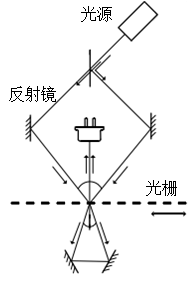
\includegraphics[width=5cm]{1-fig/佳能公司.png}
    \end{minipage}
    \label{fig:佳能公司}
  }
  \subfigure[]{
    \begin{minipage}[b]{0.40\textwidth}
      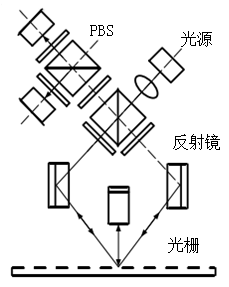
\includegraphics[width=6cm]{1-fig/佳能公司2.png}
    \end{minipage}
    \label{fig:佳能公司2}
  }
  \caption{佳能光栅位移测量结构示意图}
  \label{fig:佳能光栅位移测量结构示意图}
\end{figure}

1995年,Wen-wei Chiang 和Chih-kung Lee 在IBM公司\cite{chiang1995wavefront}提出了在光栅尺中使用像差补偿的概念,在光栅位移测量系统中也使用了双单望远镜来实现像差补偿。其结构图如图\ref{fig:美国IBM光栅读数头结构示意图}所示。像差补偿是通过球面镜和反射镜相互作用来实现的,当光源发出的激光垂直入射到光栅表面时,会发生一次衍射,此时衍射光分别进入两侧的镜头组进行补偿和反射,反射回的光会被衍射光栅进行二次衍射,通过光电探测器进行接收。
\begin{figure}[htb]
  \centering
  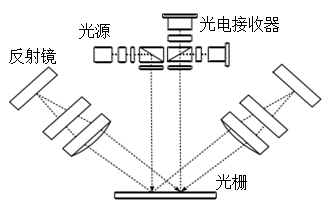
\includegraphics[width=8cm]{1-fig/IBM.png}
  \caption{美国IBM光栅读数头结构示意图}
  \label{fig:美国IBM光栅读数头结构示意图}
\end{figure}

2000年,浙江大学现代光学国家重点实验室米凤文\cite{米凤文20000}等人提出了一种新的双光束光栅测长系统,该单光栅测长结构的原理图如图 \ref{fig:浙江大学单光栅测长系统结构示意图}所示。光源通过聚光镜,反光镜垂直入射到物镜1,经物镜准直后射入光栅。±1级的两束衍射光束被物镜会聚到凹面镜上。A点的±1级衍射光被凹面镜反射,然后通过物镜在光栅B点相遇,发生二次衍射。二次衍射的光束通过物镜1会聚,然后通过小孔、半透半反镜,通过物镜2形成干涉图案,最后通过反射镜2反射到光电接收器上。当反射光栅移动,干涉条纹相应变化,对接收到的信号进行数据处理,得到光栅的实际位移。
\begin{figure}[H]
  \centering
  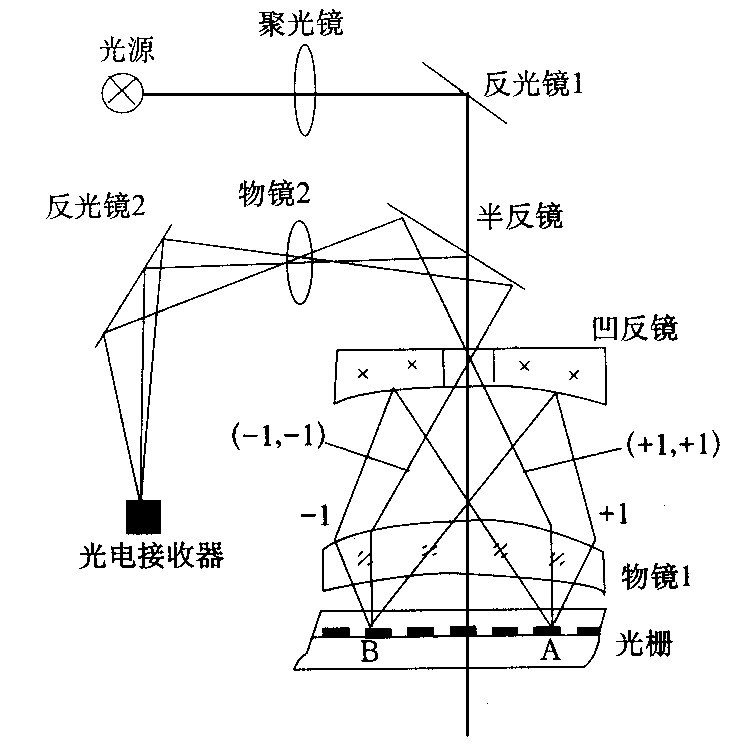
\includegraphics[width=8cm]{1-fig/浙江大学.jpg}
  \caption{浙江大学单光栅测长系统结构示意图}
  \label{fig:浙江大学单光栅测长系统结构示意图}
\end{figure}

2002年,华中科技大学郭军\cite{郭军0一种二维测长单元}等人提出了一种二维光栅测长系统,可以实现任意平面内两个正交方向的纳米级位移定位。其结构示意图如图\ref{fig:华中科技大学二维测长单元结构示意图}所示,正交衍射光栅与被测二维平面固定连接,并与被测二维平面一起移动。通过检测单元中的光学系统、光电接收装置和后续的计数细分电路,对相互正交的X、Y两个方向的位移进行准确的测量。

2017年,清华大学朱煜团队\cite{王磊杰2017超精密外差利特罗式光栅干涉仪位移测量系统,ye2019ultraprecision,ye2018translational}为应对光刻机不断提高的测量精度需求,提出了一种新型超精密外差Littrow式光栅干涉仪位移测量系统,如图\ref{fig:超精密外差利特罗式光栅干涉仪位移测量系统}所示,当光栅沿既定方向运动时,参考信号和测量信号之间的相位差可以通过相位计读出,从而推导出光栅所移动的距离。此系统的系统分辨率能达到0.41 $nm$,且由环境影响而造成的死程误差为7.59 $nm$,表明系统具有很高的环境鲁棒性。


\begin{figure}[htb]
  \centering
  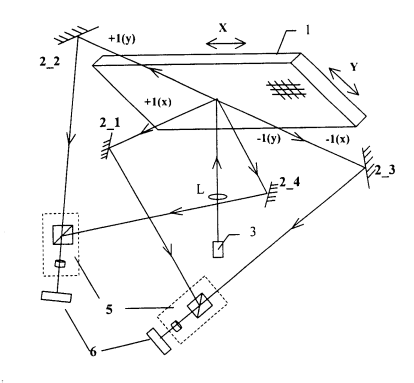
\includegraphics[width=8cm]{1-fig/华中科技大学.png}
  \caption{华中科技大学二维测长单元结构示意图}
  \label{fig:华中科技大学二维测长单元结构示意图}
\end{figure}

\begin{figure}[htb]
  \centering
  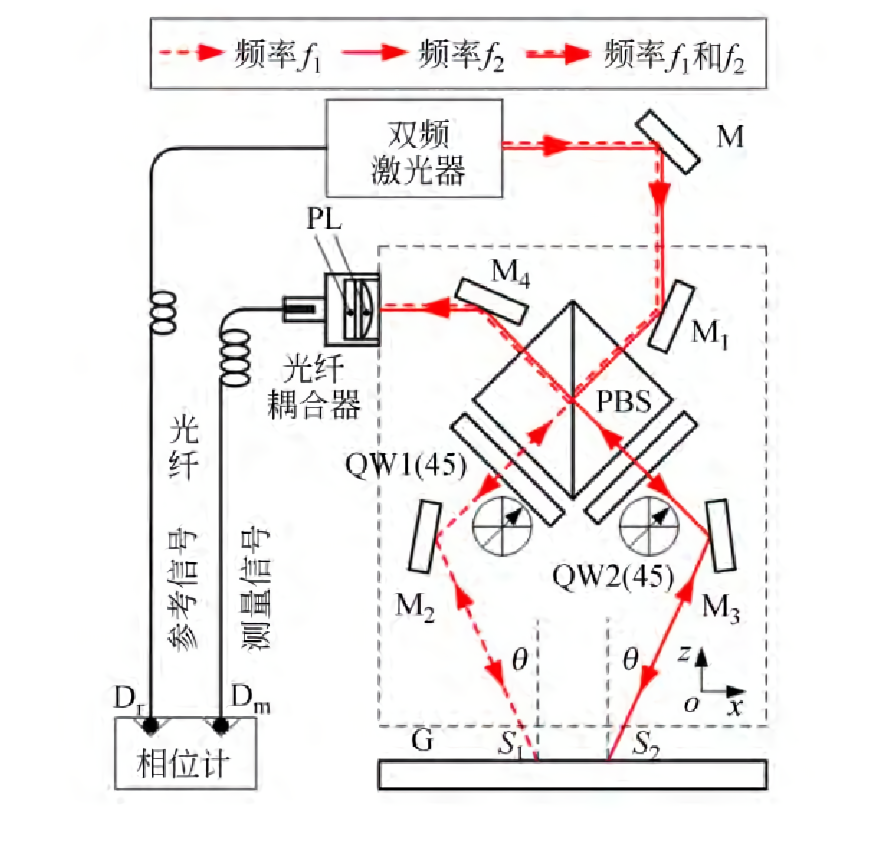
\includegraphics[width=8cm]{1-fig/清华大学.png}
  \caption{超精密外差Littrow式光栅干涉仪位移测量系统}
  \label{fig:超精密外差利特罗式光栅干涉仪位移测量系统}
\end{figure}

\begin{figure}[htb]
  \centering
  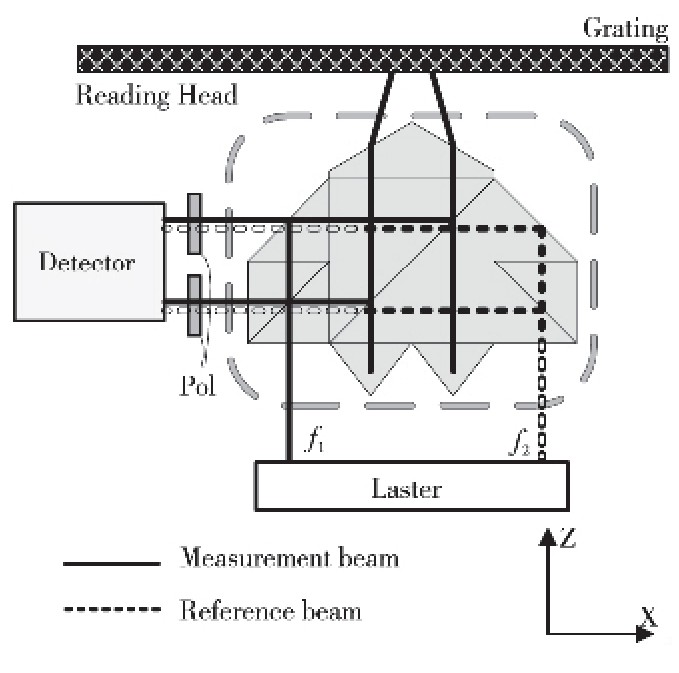
\includegraphics[width=7cm]{1-fig/桂林电子科技大学.jpg}
  \caption{平面光栅测量系统示意图}
  \label{fig:平面光栅测量系统示意图}
\end{figure}


2020年,桂林电子科技大学熊显名团队\cite{魏莉佳2020高精度平面光栅位移测量系统}采用平面光栅作为测量基准,将光栅固定在框架上,读数头安装在运动台上一起运动,当光栅于读数头之间产生相对位移时,由于多普勒效应将会产生频差,通过检测信号的频差可以得到位移值。系统示意图如图\ref{fig:平面光栅测量系统示意图}所示,实验结果表明,在全行程范围内运动时,XY向自由度的最大解算误差小于0.5 $nm$。

上文介绍了光栅位移测量系统的发展过程及其现状,可以看出,随着测量方法的不断进步,测量精度也逐渐升入到纳米级,但同时也存在一些问题,比如检测装置体积过大,不能用于高速运动台位移测量,抗环境干扰能力弱等。因此,研究一种小型化的,抗环境干扰能力强的,能用于高速运动台位移测量的光栅位移测量系统就显得尤为必要,本文将针对上述问题进行分析设计。




\subsection{光栅栅距测量}
光栅栅距作为光栅位移测量系统的基准,是指光栅两刻线之间的距离,是光栅的重要参数之一。在光栅的制造加工过程中,由于光栅刻划方法和工艺的影响光栅栅距并不是完全均匀的,存在一定的刻线误差,其累积刻线误差会被引入到测量误差中,影响测量结果的准确性,为保证测量的精度,也需要对光栅栅距进行测量。

如图\ref{fig:分光计测量栅距实验原理图}所示,一束波长为$\lambda $的平行光线照射到透射光栅后,各个狭缝产生的衍射光互相干涉,形成干涉条纹。a为光栅透光部分,b为光栅不透光部分,光栅常数即为d=a+b。根据光栅方程:
\begin{equation}
  d \sin \theta =\pm k \lambda \quad k=0,1,2, \ldots \ldots
\end{equation}
式中k为光谱级数,$\theta $为k级谱线的衍射角。通过分光计测得$\theta $,在已知$\lambda $的情况下求得光栅常数。
利用分光计测量光栅栅距\cite{倪重文2008分光计测定光栅常数,王小羊2018光栅常数测定方法探讨}操作简单,设备不复杂,但是测量精度较低,通常应用于高校课程实验中。
\begin{figure}[htb]
  \centering
  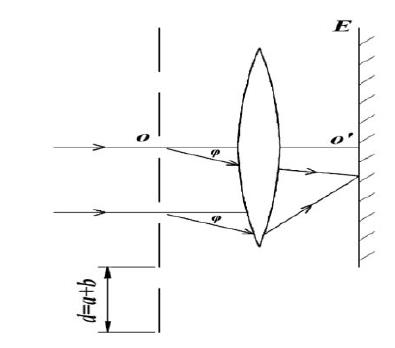
\includegraphics[width=7cm]{1-fig/分光计.jpg}
  \caption{分光计测量栅距实验原理图}
  \label{fig:分光计测量栅距实验原理图}
\end{figure}


\begin{figure}[htb]
  \centering
  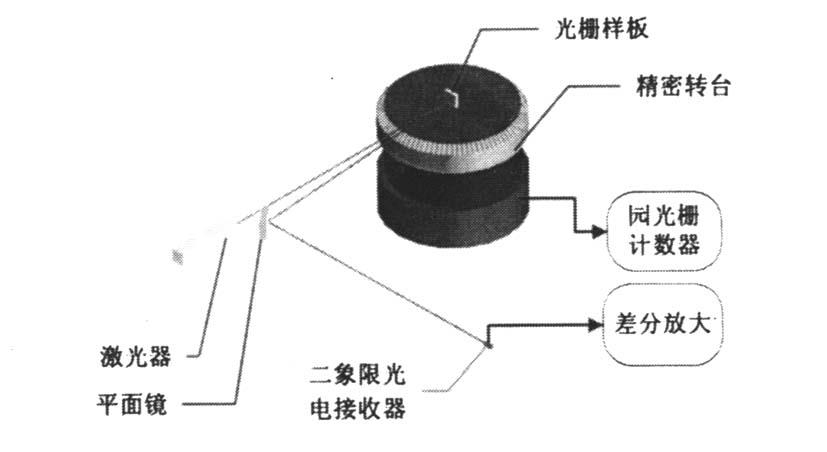
\includegraphics[width=8cm]{1-fig/Littrow衍射.jpg}
  \caption{Littrow衍射测量系统原理图}
  \label{fig:Littrow衍射测量系统原理图}
\end{figure}

2008年高思田等人采用Littrow衍射方法\cite{高思田2008纳米光栅栅距的精确测量与,lv2019fast}测量纳米光栅的栅距,其测量系统原理图如图\ref{fig:Littrow衍射测量系统原理图}所示,待测光栅置于精密转台中心,激光发射的光束以初始入射角$ \gamma $照射到光栅表面。由于衍射效应,会形成衍射条纹。转动精密转台,使0级和±1级衍射光依次进入二象限光电接收器,当差分放大器的读数为0时,记录此时转盘的旋转角度为$ \alpha $。根据光栅方程
\begin{equation}
  d(\sin (\alpha+\gamma )+\sin (\alpha- \gamma ))=k \cdot \lambda
\end{equation}
\begin{equation}
  2d \sin\alpha \cos\gamma  =k \cdot \lambda
\end{equation}
给定已知的激光波长$ \lambda $和旋转角$\alpha  $以及初始入射角$\gamma  $,可得到光栅栅距为:
\begin{equation}
  p=\frac{k \lambda}{2 \sin \alpha \cos \gamma}
\end{equation}



2015年Yancong Lu等人利用数字图像相关技术\cite{lu2016pitch,chen2014novel}对光栅栅距进行评估,其测量原理图如图\ref{fig:CCD测量系统原理图}所示,激光光源经透镜反射后垂直照射到位移台上的光栅上,位移台上的光栅行程为300$mm$,分辨率为0.25$um$。光栅经过数值孔径(NA)为0.25的物镜在CCD相机上成像。在图像上可以观察到光栅沟槽和不透光部分。随后计算机对图像进行处理和分析,最后利用DIC技术对光栅栅距进行计算。图\ref{fig:CCD扫描光栅图像}展示了CCD相机下得到的光栅图像。

\begin{figure}[htb]
  \centering
  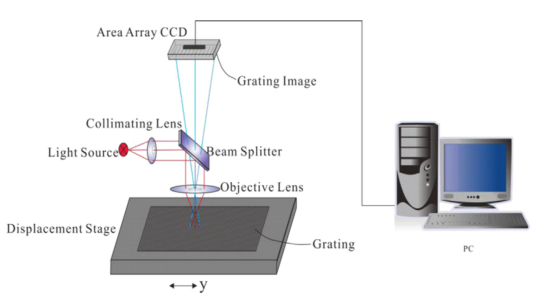
\includegraphics[width=7cm]{1-fig/CCD.png}
  \caption{CCD测量系统原理图}
  \label{fig:CCD测量系统原理图}
\end{figure}

\begin{figure}[htb]
  \centering
  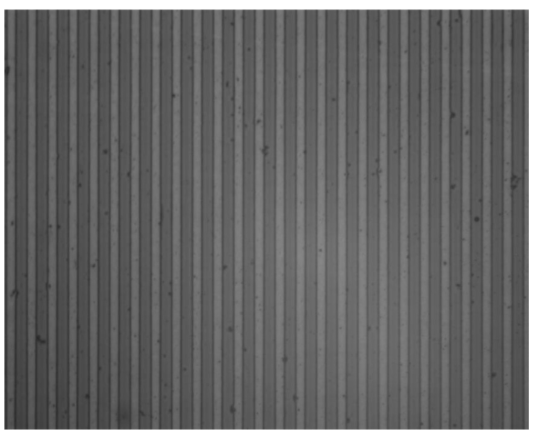
\includegraphics[width=7cm]{1-fig/光栅图像.png}
  \caption{CCD扫描光栅图像}
  \label{fig:CCD扫描光栅图像}
\end{figure}


2018年陈云云等人\cite{陈云云2019一种测量光栅常数的系统}发表了一篇基于莫尔条纹测量光栅常数的专利。该系统如图\ref{fig:基于莫尔条纹的栅距测量系统}所示,光源发出的探测光通过扩束准直系统成像得到莫尔条纹,该莫尔条纹经过图像采集系统采集转化为与所述莫尔条纹宽度、间隔相等的条纹状图,该条纹状图上的条纹间隔即为莫尔条纹的间隔D。根据如下公式计算得到光栅的光栅常数:
\begin{equation}
  D=\frac{d_{1} d_{2}}{\left(d_{1}^{2}+d_{2}^{2}-2 d_{1} d_{2} \cos \theta\right)^{\frac{1}{2}}}
\end{equation}

其中D为莫尔条纹的间隔,$d_{1}$和$d_{2}$分别表示为标准光栅和待测光栅的光栅常数,$\theta $是两个光栅之间的角度。标准光栅的光栅常数$d_{1}$是已知的,只需求得夹角$\theta $就能得到待测光栅的光栅常数$d_{2}$。
\begin{equation}
  \mathrm{d_{2}}=\frac{2 D^{2} d_{1} \cos \theta \pm \sqrt{-2 D^{4} d_{1}^{2}+4 D^{2} d_{1}^{4}+2 D^{4} d_{1}^{2} \cos 2 \theta}}{2\left(D^{2}-d_{1}^{2}\right)}
\end{equation}

\begin{figure}[htb]
  \centering
  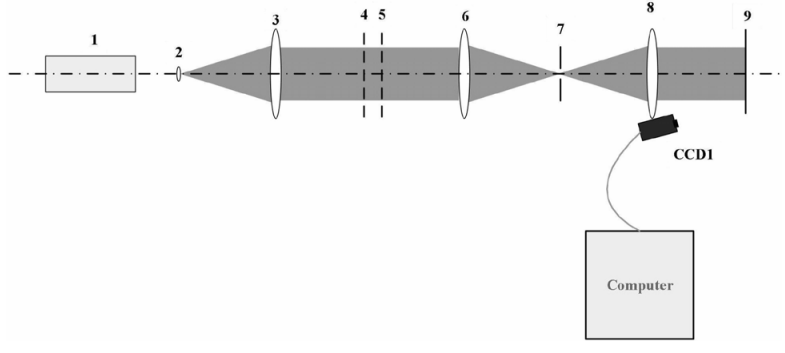
\includegraphics[width=10cm]{1-fig/莫尔条纹.png}
  \caption{基于莫尔条纹的栅距测量系统}
  \label{fig:基于莫尔条纹的栅距测量系统}
\end{figure}


2020年路陈陈\cite{路陈陈2020平面波导光栅常数检测装置的研究}提出了一种平面波导光栅常数的检测装置,该装置检测示意图如图\ref{fig:平面波导光栅的测量装置}。激光光束以$\theta $入射到平面波导光栅后,一部分光在光栅内进行全反射,一部分光由光栅透射出去形成出射光斑,通过CCD扫描光斑传入计算机进行处理,即可得到出射光斑的距离为x,平面波导光栅的计算公式如下:
\begin{equation}
  d=\frac{m \lambda}{n_{2}\left[\sin \theta+\sin \left(\arctan \frac{x}{2 t}\right)\right]}
\end{equation}
其中$\lambda $为入射光波长,m为衍射级次均已知,当激光光束垂直入射时,光线入射角$\theta $为0,因此我们只需测得平面波导光栅的折射率$ n_{2}$,厚度$ t$和出射光斑的距离$ x$即可求得平面波导光栅的栅距$ d$。
\begin{figure}[htb]
  \centering
  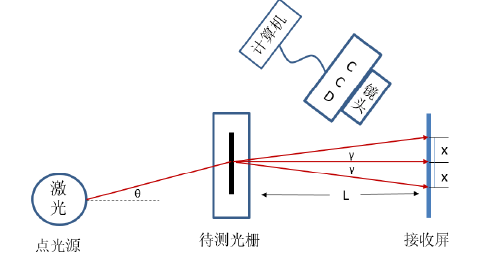
\includegraphics[width=9cm]{1-fig/平面波导光栅的测量装置.png}
  \caption{平面波导光栅的测量装置}
  \label{fig:平面波导光栅的测量装置}
\end{figure}

上文主要介绍了光栅栅距测量的一些方法,在以光栅栅距作为测量基准的系统中,对光栅栅距进行准确的测量还是很有必要的。分析现有的栅距测量方法,可以分为两大类,直接测量法和间接测量法。直接测量法一般使用高精度的设备,如扫描显微镜或者CCD相机,对栅距进行直接测量;间接测量法一般将栅距转化为其他变量进行测量,最后在反推回光栅栅距。现有的测量方法测量精度大多不能达到纳米级,且通常检测流程繁琐。本文针对上述问题进行研究,致力于提出一种测量精度高,无接触式的测量方法。



\section{主要研究内容和结构安排}
\subsection{主要研究内容}
本文针对超精密位移测量中测量精度、测量速度和检测装置体积等问题,开展基于外差干涉技术的纳米光栅位移测量系统的研究,实现超精密位移检测。本文将从测量系统的设计、测量系统的实验、误差分析、光栅栅距的测量和误差补偿五个方面展开研究。

1)外差式光栅位移测量系统的设计和分析。为实现纳米级位移检测,本文对光路结构进行了分析和改进,基于光栅衍射特性、衍射干涉原理和光学多普勒效应重新设计了光源模块和读数头模块,将所有的光学元件进行集成化,实现了结构的小型化。所设计的光栅位移测量系统相较于传统超精密位移测量方法,实现了亚纳米级精度的测量同时控制了结构的体积,具有较大的进步。

2)测量系统的实验和误差分析。对所设计的测量系统进行实验平台的搭建,对光栅位移测量系统各方面进行实验测试,对系统的误差来源进行分析,包括光栅非理想误差、几何误差、环境误差三部分。针对环境误差中的非共光程误差进行实验测量。

3)光栅栅距的测量。针对测量系统中的光栅非理想误差,分析现有的栅距测量方法,提出一种无接触式,测量精度高的方法。并进行实验验证,与基于扫描显微镜的方法结果进行对比,验证方法的可行性。

4)光栅位移测量系统的误差补偿。针对测量系统的误差分析和光栅栅距的测量,使用三次样条插值法对误差进行补偿,并与基于最小二乘法的方法进行对比实验,结果表明补偿效果良好,明显提升了测量系统的精度。


\subsection{论文结构安排}
本论文共分为六章:

第一章为绪论。首先介绍了论文的研究背景和意义,然后对光栅位移测量方法进行了系统综述,给出比较有代表性的光栅位移测量系统的光路结构,阐述其原理。其次对光栅栅距的测量方法进行综述,分析了国内外测量方法的原理及其精度。最后概述了本文的主要研究内容,并阐述了论文的章节架构。

第二章为光栅位移测量原理。本章对光栅位移测量系统的原理进行了梳理,首先介绍了光栅的理论基础,其次从光路光程推导和多普勒频移两方面分析了光栅位移测量的原理,最后
介绍了拍频现象产生的原理,由此引申出本文所使用的外差干涉技术,对其进行说明和推导,便于后文设计工作的展开。

第三章为外差式光栅位移测量系统的光路设计和分析。本章首先介绍了光路系统的设计原则,引出本文所设计的光栅位移测量系统的整体方案,将其分为两大部分,光源模块的设计和读数头模块的设计。对整个系统的光路进行偏振光学推导,阐述详细的测量原理,为第四章的实验搭建和测试做铺垫。

第四章为光栅位移测量系统实验及其误差分析。本章首先介绍了光路调试与安装的主要步骤,组装光源模块和读数头模块,构建整个系统进行实验。性能测试部分主要分为短行程位移测试,长行程位移测量和稳定性测量。最后对整个光栅位移测量系统的误差进行分析,主要从光栅非理想误差,几何误差,测量环境误差三部分进行说明,对测量环境误差中的光路非共光程误差进行实验测量,分析其对整个系统的影响。

第五章光栅栅距测量及其误差修正。本章承接第四章误差分析的内容,对光栅非理想误差进行详细说明,提出了一种新的光栅栅距测量方法,主要基于激光干涉原理和光栅衍射原理,在光栅运动过程中将光栅栅距转换为干涉仪和光栅位移对比量。最后进行实验验证,并与基于SEM的方法进行对比,验证方法的可行性。同时采用三次样条插值法来对实验结果进行补偿,并与基于最小二乘法的方法进行对比实验,证明了补偿方法的可行性。

第六章总结和展望。本章总结了全文所作的工作,并对后续研究进行了展望。

\begin{figure}[H]
  \centering
  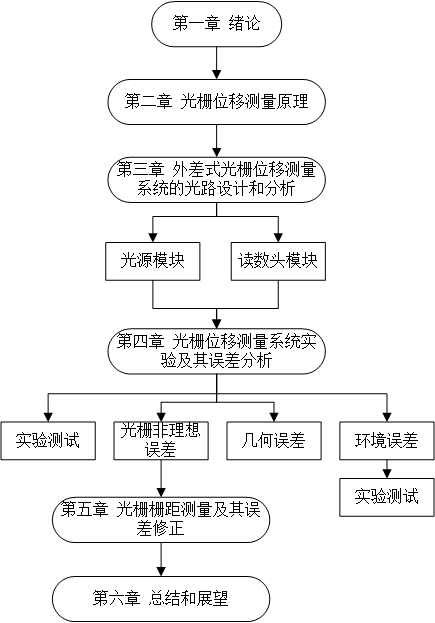
\includegraphics[width=10cm]{1-fig/章节结构图.png}
  \caption{章节结构图}
  \label{fig:章节结构图}
\end{figure}


\chapter{光栅位移测量原理}
\section{光栅理论基础}
光栅\cite{石顺祥2000物理光学与应用光学,palmer2005diffraction}通常是指由大量等间距的平行狭缝构成的光学元件。但随着光栅制造技术的发展,光栅不再局限于狭缝的概念。现在广义上的光栅又可定义为可以使得入射光相位或者振幅受到周期性调制的光学元件。按照光栅对入射光的调制方法不同可以分为振幅光栅和相位光栅,按照工作方式可分为反射光栅和透射光栅。透射式光栅是在一块光学材料上等间距的刻划出大量平行凹痕,凹痕处不透光,两凹痕之间的部分则是可以透光的狭缝。反射光栅则是在反射镜上进行刻划,在凹痕上发生漫反射,未刻划的部分则在反射光的方向上发生衍射。本文的光栅位移测量系统采用的是反射光栅,如图\ref{fig:光栅示意图}所示是光栅的示意图。
\begin{figure}[H]
  \centering
  \subfigure[透射光栅]{
    \begin{minipage}[b]{0.4\textwidth}
      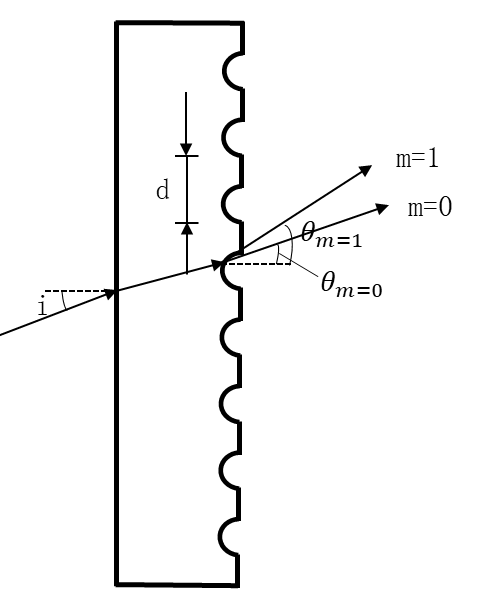
\includegraphics[width=5cm]{2-fig/透射光栅示意图.png}
    \end{minipage}
    \label{fig:透射光栅}
  }
  \subfigure[反射光栅]{
    \begin{minipage}[b]{0.4\textwidth}
      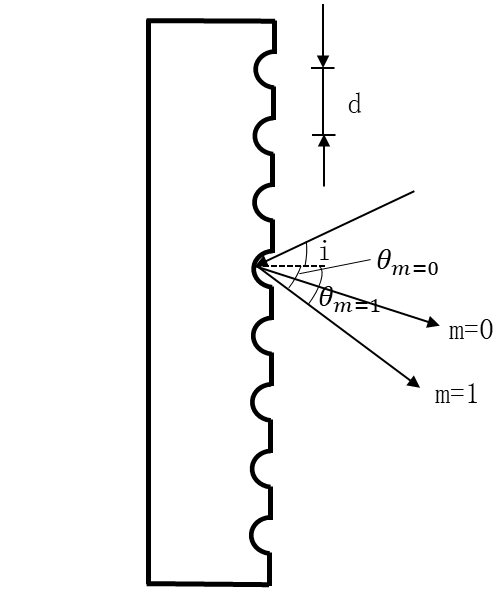
\includegraphics[width=5cm]{2-fig/反射光栅示意图.png}
    \end{minipage}
    \label{fig:反射光栅}
  }
  \caption{光栅示意图}
  \label{fig:光栅示意图}
\end{figure}

\section{光栅位移测量原理}
\subsection{光栅衍射特性}
如图\ref{fig:光栅衍射特性}所示,当激光光束以$\alpha $角入射到反射光栅表面,将会发生衍射,入射角和衍射角满足光栅衍射方程:
\begin{equation}
  D(\sin \alpha \pm\sin \theta)=k \cdot \lambda \quad k=0,\pm1,\pm2, \ldots
\end{equation}
其中$\alpha $为入射角,$\theta $ 为衍射角,$D$为光栅栅距,$\lambda $ 为入射激光波长,$k$为衍射级次。当入射光和$k$级衍射光处于光栅面的法线同一侧时,上式取正号;当入射光和$k$级衍射光处于光栅面的法线两侧时,上式取负号。按照同样的推导方法可以证明透射光栅也满足上述光栅衍射方程。

当$k$为0时,由上式可以得到,零级衍射光和入射光处于光栅法线的两侧,且衍射角和入射角相等;当$\alpha $为0时,即激光光束垂直入射到光栅表面时,$+k$级和$-k$级衍射光会处于光栅法线的两侧,且与光栅法线的夹角相等。
\begin{figure}[H]
  \centering
  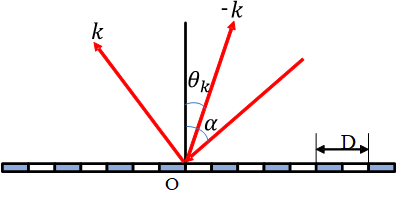
\includegraphics[width=8cm]{2-fig/光栅衍射特性.png}
  \caption{光栅衍射特性}
  \label{fig:光栅衍射特性}
\end{figure}

\subsection{光路光程推导}
光程差定义为两束光到达某个点的光程之差,光程差与相位差之间的关系可以由下式得到:
\begin{equation}
  \Delta \phi =2 \pi / \lambda \times \Delta L
\end{equation}

当光栅以速度$\upsilon $沿运动方向位移时,运动前和运动后的两束光之间会产生光程差,由此导致相位差,位移信息被保存在相位差中,通过解调可以得到位移值。通过分析光栅移动前后光程的变化得到光栅位移和相位变化之间的关系。

激光光束以初始入射角$\alpha $入射至反射光栅表面,当光栅沿运动方向移动$\Delta s$时,+1级的衍射光的光程变化如图\ref{fig:+1级衍射光光程}所示,可以得到光程与运动距离的关系为:
\begin{equation}
  \Delta L_{i}=\Delta S \cdot \sin \alpha
\end{equation}
\begin{equation}
  \Delta L_{+1}=\Delta S \cdot \sin \theta_{+1}
\end{equation}
由此可得+1级衍射光的相位变化与光栅位移的关系:
\begin{equation}
  \begin{aligned}
    \Delta \varphi_{y+1} & =\frac{2 \pi}{\lambda} \cdot \Delta L =\frac{2 \pi}{\lambda} \cdot\left(\Delta L_{i}-\Delta L_{+1}\right) =\frac{2 \pi}{D} \cdot \Delta S
  \end{aligned}
\end{equation}
\begin{figure}[H]
  \centering
  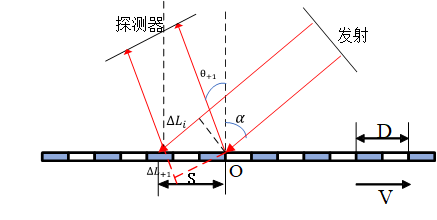
\includegraphics[width=8cm]{2-fig/+1级光程差.png}
  \caption{+1级衍射光光程}
  \label{fig:+1级衍射光光程}
\end{figure}

同理分析-1级的衍射光光程变化如图\ref{fig:-1级衍射光光程}所示,其光程与运动距离的关系为:
\begin{equation}
  \Delta L_{i}=\Delta S \cdot \sin \alpha
\end{equation}
\begin{equation}
  \Delta L_{-1}=\Delta S \cdot \sin \theta_{-1}
\end{equation}
此时-1级衍射光的相位变化与光栅位移的关系:
\begin{equation}
  \begin{aligned}
    \Delta \varphi_{y-1} & =\frac{2 \pi}{\lambda} \cdot \Delta L =\frac{2 \pi}{\lambda} \cdot\left(\Delta L_{+1}+\Delta L_{i}\right) =-\frac{2 \pi}{D} \cdot \Delta S
  \end{aligned}
\end{equation}
\begin{figure}[H]
  \centering
  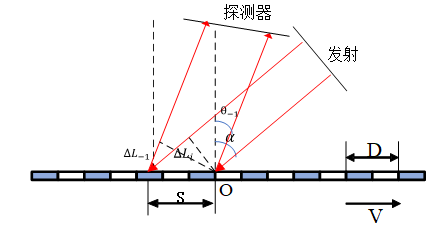
\includegraphics[width=8cm]{2-fig/-1级光程差.png}
  \caption{-1级衍射光光程}
  \label{fig:-1级衍射光光程}
\end{figure}
综上所述,当光栅沿运动方向移动$\Delta S$时,±1级的衍射光相位差与运动位移之间的关系如下:
\begin{equation}
  \Delta \varphi=\Delta \varphi_{y+1}-\Delta \varphi_{y-1}=\frac{2 \pi}{D} \cdot \Delta S-(-\frac{2 \pi}{D} \cdot \Delta S)=\frac{4 \pi}{D} \cdot \Delta S
\end{equation}

在相位 $ \Delta \phi $中记录了待测物体的位移信息,相位的变化又可通过板卡来进行测量,再经过计算机处理即可得到待测物体位移量。


\subsection{多普勒频移}
多普勒效应\cite{giordano2012college}是奥地利物理学家和数学家Doppler于1842年提出的理论,其主要内容如图\ref{fig:多普勒效应示意图}所示:当声源与接收声源的物体之间发生相对运动时,声源的频率会发生改变。当接收物体远离声源时,接收到的声音频率会变低,波长变长;当接收物体靠近声源时,接收到的声音频率会变高,波长变短。多普勒效应的公式\cite{shi2018superlight}如下:
\begin{equation}
  f^{\prime}=\left(\frac{v \pm v_{o}}{v \mp v_{s}}\right) f
\end{equation}
其中,$f^{\prime}$是接收声源的物体所观测到的频率,$f$是声源发射时在介质中的原始频率,$\upsilon $是波在介质中的运动速度,$v_{o}$是接收声源的物体相对于介质的移动速度,如果它靠近发射源,前面的操作符号为+号,否则为-号,$v_{s}$为声源发射时相对于介质的移动速度,如果靠近观察者,前面的操作符号为-号,否则为+号。
\begin{figure}[htb]
  \centering
  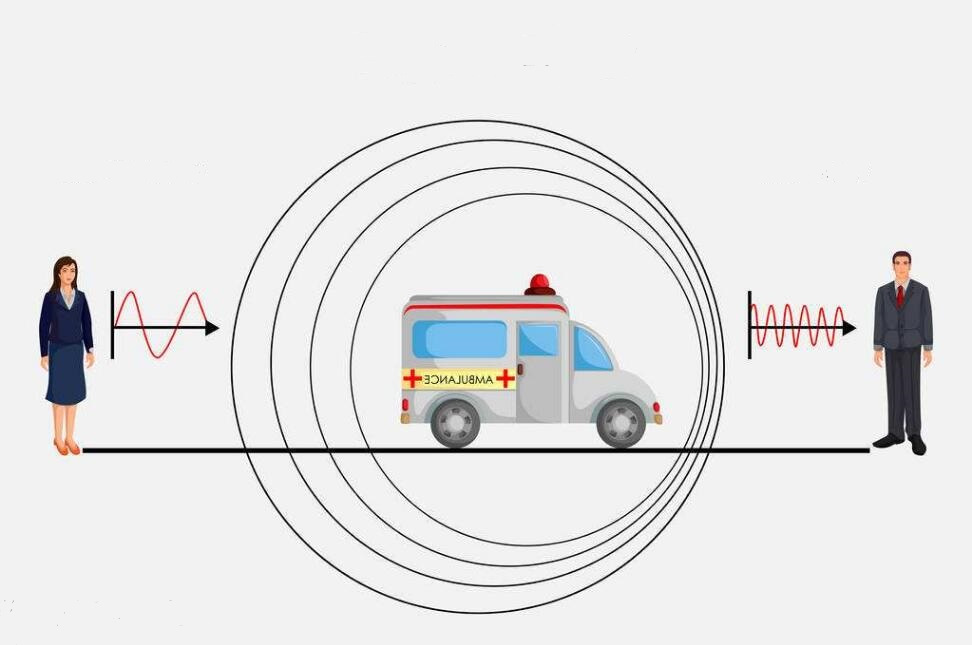
\includegraphics[width=7cm]{2-fig/多普勒效应.jpeg}
  \caption{多普勒效应示意图}
  \label{fig:多普勒效应示意图}
\end{figure}

具有波动性的光也会出现这种效应。在光栅位移测量系统中,激光光源作为原始发射源,反射光栅作为接收物体,当激光光源照射到反射光栅后,产生衍射光。衍射光栅位置变化时就会产生多普勒效应,具体表现在$\pm 1$级衍射光的频率发生变化。

如图\ref{fig:多普勒频移分析}所示,当激光光源作为原始发射源,以入射角 $ \alpha $入射至反射光栅,此时反射光栅作为接收物体,其运动速度为$ \upsilon $,栅距为$D$。相当于激光光束在以$\operatorname{vsin} \alpha$的速度接近$ O $点,此时根据上述多普勒效应,将$ O $点视为观察者,发射源相对于介质的移动速度靠近观察者,操作符取+号,在光栅表面$ O $观察到的光频率变为:
\begin{equation}
  f^{\prime}=\left(\frac{1+v \sin \alpha}{c}\right)f
\end{equation}

当衍射光以出射角$ \theta_{k} $从光栅表面射出时,相当于光源以$ v \sin \theta_{k} $的速度沿出射方向接近 $ k $ 点。此时根据上述多普勒效应,将$ k $ 点视为观察者,发射源相对于介质的移动速度靠近观察者,操作符取+号,在 $ k $ 点观测到的各级次衍射光对应的频率为:
\begin{equation}
  \begin{aligned}
    f^{\prime \prime}=f^{\prime}\left(1+\frac{v \sin \theta_{k}}{c}\right) & =f\left(1+\frac{v \sin \alpha}{c}\right)\left(1+\frac{v \sin \theta_{k}}{c}\right) \\& =f\left[1+\frac{v}{c}\left(\sin \alpha+\sin \theta_{k}\right)+\frac{v^{2}}{c^{2}} \sin \alpha \sin \theta_{k}\right]
  \end{aligned}
\end{equation}
由于$ \upsilon \ll c$,忽略上式中高次项的影响,并将$c=\lambda f^{\prime}$和光栅方程$D(\sin \alpha+\sin \theta)=k \lambda$代入,可得到多普勒频移$ \Delta f $:
\begin{equation}
  \Delta f=f^{\prime \prime}-f=\frac{v}{\lambda}\left(\sin \alpha+\sin \theta_{k}\right)=\frac{k v}{D}
\end{equation}
由上式可以看出,衍射光栅的多普勒频移与光栅栅距$D$成反比关系,与光栅的运动速度$ \upsilon $和衍射级次 $ k $ 成正比关系,而与入射光的角度$ \alpha $和入射光的波长$\lambda $无关。此时 $ \pm k $级衍射光的频率差可以表示为:
\begin{equation}
  \Delta f=f_{+k}-f_{-k}=f^{\prime}+\frac{k v}{D}-\left(f^{\prime}-\frac{k v}{D}\right)=2 k \frac{v}{D}
\end{equation}
两束衍射光之间的相位差:
\begin{equation}
  \Delta \phi=\int_{0}^{t} 2 \pi \Delta f d t=\int_{0}^{t} 4 k \pi \frac{v}{D} d t=4 k \pi \frac{\Delta S}{D}
\end{equation}

在相位 $ \Delta \phi $中记录了待测物体的位移信息,相位的变化又可通过板卡来进行测量,再经过计算机处理即可得到待测物体位移量。

\begin{figure}[H]
  \centering
  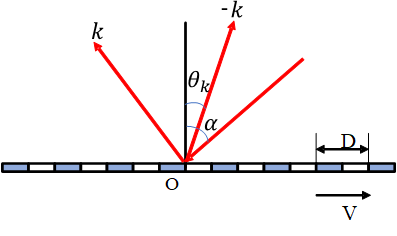
\includegraphics[width=0.5\textwidth]{2-fig/多普勒频移分析.png}
  \caption{多普勒频移分析}
  \label{fig:多普勒频移分析}
\end{figure}

\section{外差干涉原理}
\subsection{拍频现象}
当同一方向上频率差异不大的两个简谐波叠加时,叠加产生的波形的幅值将随时间呈现周期性变化,具体表现为幅值忽高忽低,这一现象也被称之为“拍”。单位时间内出现的拍数称为拍频,也即一强一弱的变化次数,在波形上表现为幅值变化的频率。通常情况下,这两个简谐波的频率差不大,叠加产生的波形的频率与原始简谐波的频率相近,但是当我们计算拍频时就可以发现,拍频的频率远低于原始简谐波的振动频率。由此可以看出,当两个频率相差不大的简谐波进行叠加时,由于“拍”现象的存在,高频原始简谐波中的频率信号被转移到低频叠加波的拍频信号中,由原本难以测量的高频信号变为易于测量的低频拍频信号,大大减少了测量的难度。

假设两个简谐波的原始方程为:
\begin{equation}
  \begin{aligned}
     & x_{1}(t)=A_{1} \cos \left(\omega_{1} t+\varphi\right) \\
     & x_{2}(t)=A_{2} \cos \left(\omega_{2} t+\varphi\right)
  \end{aligned}
\end{equation}
假设$A_{1}=A_{2}=A$,且$|\omega_{1}-\omega_{2}|<<\omega_{1}+\omega_{2}$时,根据和差化积公式,它们叠加后形成拍的波形方程为:
\begin{equation}
  \begin{aligned}
    x(t) & =x_{1}(t)+x_{2}(t)=A\left[\cos \left(\omega_{1} t+\varphi\right)+\cos \left(\omega_{2} t+\varphi\right)\right]      \\
         & =2 A\left|\cos \frac{\omega_{2}-\omega_{1}}{2} t\right| \cos \left(\frac{\omega_{1}+\omega_{2}}{2} t+\varphi\right)
  \end{aligned}
\end{equation}
式中 $ 2A\left|\cos \frac{\omega_{2}-\omega_{1}}{2} t\right| $为叠加后的拍的幅值。拍频定义为单位时间内合振动振幅强弱变化的次数,即
\begin{equation}
  f=\left|\frac{\omega_{2}-\omega_{1}}{2 \pi}\right|=\left|f_{2}-f_{1}\right|
\end{equation}

波 $x_{1}$、$x_{2}$ 以及两个简谐波叠加后产生的波$x$如图\ref{fig:拍频现象}所示。根据上式可以看出,拍频信号的频率为两个简谐波频率的差值,在波形上表现为周期性变换的结构。由此也可看出,当其中一个简谐波的相位发生变化,拍频信号的相位也会发生相同的变化,这也就将高频信号的信息转移到了拍频信号中,保留了原始高频信号的相位信息\cite{张志平2022激光外差干涉技术在光刻机中的应用}。

对于激光位移测量领域,当前的光电探测器无法检测到频率过高的信号(原始信号为$10^{14} $Hz量级),但是可以检测到低频信号,也即可以检测到两个高频信号叠加产生的低频拍频信号($10^{2} $Hz量级)。因此,现有的激光位移测量系统大多应用了拍频技术,发展成为激光外差干涉技术。

\begin{figure}[H]
  \centering
  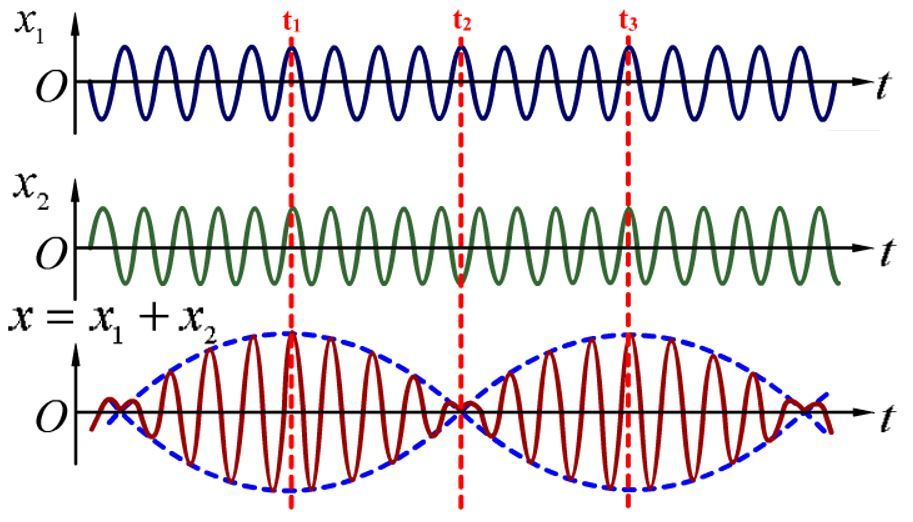
\includegraphics[width=0.5\textwidth]{2-fig//拍频现象.jpg}
  \caption{拍频现象}
  \label{fig:拍频现象}
\end{figure}

\subsection{外差干涉技术}
传统的干涉位移测量装置的基本原理是:单频激光光源通过一定的光路结构被分为参考光和测量光,在测量光中携带了位移信息,再通过光路结构进行叠加,产生干涉,形成干涉条纹,通过干涉条纹中的光强变化来推导被测物体的位移变化。采用传统的干涉位移测量装置,形成的干涉条纹易受空气中的环境干扰,影响条纹质量。此种方法测量精度能够达到亚微米级,能够满足一般的测量精度,但距离光刻机内部精度要求仍相差甚远,为了获得纳米级精度甚至更高的分辨率,就需要应用到拍频技术,也即外差干涉技术。

外差干涉法是一种测量光的相位变化的方法。使用外差干涉仪时,两个输入光束都具有特定的频率或波长,当光束进行叠加干涉后,形成的干涉信号是随时间和相位变化的拍频。在位移测量过程中,拍频信号的相位中记录了被测物体的位移信息,剩下的工作就是通过相对应的相位解调技术求得被测物体的位移量。采用外差干涉法来测量位移信息,由于直接对信号来进行叠加和解调,不涉及光强强弱的变化,因此对于环境中的影响因素有着较为良好的抗干扰能力,具体表现为测量精度能够达到纳米级精度,满足光刻机内部位移测量精度要求。

外差干涉仪的基本结构如图\ref{fig:外差干涉原理图}所示。一外差光源的光束被分光镜BS分为反射光透射光两部分。反射光通过偏振片后作为参考光被光电探测器接收;透射光进入待测系统产生相位差,被光电探测器接收进行比较,解调出位移信息。
\begin{figure}[H]
  \centering
  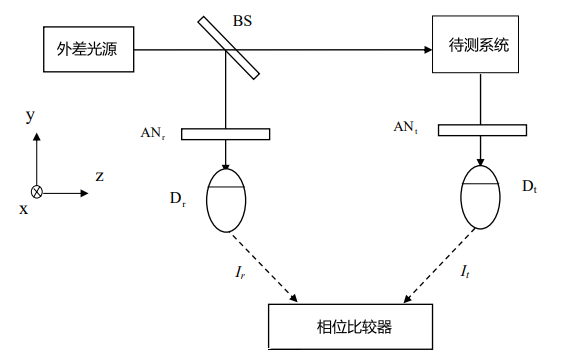
\includegraphics[width=10cm]{2-fig/外差干涉原理图.png}
  \caption{外差干涉原理图}
  \label{fig:外差干涉原理图}
\end{figure}

假设图 \ref{fig:外差干涉原理图} 输入的参考光和测量光的电场形式分别为:
\begin{equation}
  E_{1}(t)=A_{1} \exp \left(i \omega_{1} t\right)
\end{equation}
\begin{equation}
  E_{2}(t)=A_{2} \exp \left[i\left(\omega_{2} t+\phi\right)\right]
\end{equation}
其中,$ A_{1}$和$ A_{2}$表示光的振幅,$\omega_{1}$和$\omega_{2}$表示其角频率,$\phi $为待测物体运动引起的相位差,且:
\begin{equation}
  \omega_{1}=\omega_{0}+\Delta \omega / 2
\end{equation}
\begin{equation}
  \omega_{2}=\omega_{0}-\Delta \omega / 2
\end{equation}

当两束光重叠后产生的拍频信号被光电探测器接收,在光电探测器上得到的光强为:
\begin{equation}
  \begin{aligned}
    I(t)\propto & \left|E_{1}+E_{2}\right|^{2}= A_{1}^{2}+ A_{2}^{2}+\left[A_{1}^{2} \cos \left(2 \omega_{1} t\right)+A_{2}{ }^{2} \cos \left(2 \omega_{2} t+\phi\right)\right] \\
                & +2A_{1} A_{2} \cos \left[\left(\omega_{1}+\omega_{2}\right) t+\phi\right]+ 2A_{1} A_{2} \cos \left[\left(\omega_{1}-\omega_{2}\right) t+\phi\right]
  \end{aligned}
\end{equation}
其中 $\left[A_{1}^{2} \cos \left(2 \omega_{1} t\right)+A_{2}{ }^{2} \cos \left(2 \omega_{2} t+\phi\right)\right] $和 $2A_{1} A_{2} \cos \left[\left(\omega_{1}+\omega_{2}\right) t+\phi\right] $ 部分为高频项,由于光电探测器不能探测到高频信号,因此该高频部分不会被检测到,此时剩余部分的信号形式为:
\begin{equation}
  \begin{aligned}
    I(t) & =A_{1}^{2}+A_{2}^{2}+2A_{1} A_{2} \cos \left[\left(\omega_{1}-\omega_{2}\right) t+\phi\right] \\
         & \propto I_{1}+I_{2}+2 \sqrt{I_{1} I_{2}} \cos (\Delta \omega t+\phi)
  \end{aligned}
\end{equation}
设$I_{0}=I_{1}+I_{2}$,则公式可以写为:
\begin{equation}
  I(t)=I_{0}[1+V \cos (\Delta \omega t+\phi)]
\end{equation}
其中,V 为对比度,可以表示为:
\begin{equation}
  V=\frac{2 \sqrt{I_{1} I_{2}}}{I_{1}+I_{2}}
\end{equation}

由上式可知,外差干涉法主要利用外差光源发射的两束频差不大的光束进行干涉测量,形成的干涉信号是随时间和相位变化的拍频,其频差为$\Delta \omega$ ,在相位$ \phi$中记录了要测量的位移信息,通过测量拍频信号的相位变化可以计算位移测量值。


\section{本章小结}
本章主要介绍了光栅位移测量的基本理论。首先阐述了光栅的基础知识,给出光栅的定义分类以及本实验所选用的衍射光栅。随后分析光栅位移测量的原理,其中包括光栅衍射特性、光路光程推导、多普勒频移,给出公式推导和原理图,在相位$ \phi$中记录了要测量的位移信息,通过测量拍频信号的相位变化可以计算位移测量值。最后介绍了本文所采用的外差干涉测量的基本原理,包含拍频现象及外差干涉光强推导,为后文光栅位移测量系统光路设计提供了基础。


\chapter{外差式光栅位移测量系统光路设计和分析}
\section{光栅位移测量系统的设计原则}
在进行外差式光栅位移测量系统的光路设计时,为了使系统的分辨率和精度更高,应尽量遵循以下原则:

1)尽量满足高光强的原则。在进行光路设计的过程中尽量选择光强较大的级次进行衍射,这样既方便了调试过程,也使得光电探测器检测到的光束强度能够达标,避免因光强较弱影响到实验结果。

2)利用高阶衍射原理。由上文对多普勒效应的分析表明,被测光的频率差与衍射级成正比。衍射级越高,光路的倍频越多,可以获得更高的分辨率。因此在保证高光强的原则下,应尽量选择更高级次的衍射,以获得更高的精度。

3)使用多次衍射原理。由上文对多普勒效应的分析表明,在经历一次衍射后就会产生一次多普勒频移,因此在进行光路设计时,应充分利用光栅的衍射特性,采用二次衍射光作为测量光,叠加两次多普勒频移,提高系统的分辨率。

4)采用对称原则。在设计光源模块时,两束光的光路应尽量保持对称,使得两束光的光程差尽可能的小。如果采用对称原则,此时外界环境因素对两束光的影响是一样的,在一定程度上能够减少环境干扰导致的误差。

5)偏光光学理论的应用。设计的光源模块产生的外光源是偏振方向相互垂直的线偏振光,在光路设计的过程中,应合理应用偏振光学理论,通过摆放偏振分光棱镜,1/4波片等偏振器件,控制光路的偏振方向,获得更好的信号,方便后续处理数据。


\section{外差式光栅位移测量系统整体方案}
整个光栅位移测量系统主要由光源模块,读数头,反射光栅,运动台,信号处理,上位机组成。其中反射光栅作为测量基准固定在运动台上,读数头与反射光栅相平行。光源模块发出的外差光源经读数头射向光栅,参考光束和测量光束通过保偏光纤接入信号处理板卡,由上位机进行处理显示结果。

系统的测量光路如图\ref{fig:光栅位移测量系统光路图}所示,主要包括光源,反射镜,分光镜,角锥棱镜,反射光栅。其中BS代表分光镜,M表示反射镜,P代表角锥棱镜。由图\ref{fig:光栅位移测量系统光路图}可知,光源模块发出频率为$ f_{1}$和$ f_{2}$的两束光,这两束光是相互垂直并且偏振的,当倾斜入射到分光镜BS后,又可分为两束光,其中透射光由光纤传输到信号处理板卡上,作为参考信号。反射光垂直入射到反射光栅上发生一次衍射,正负一级衍射光沿法线对称角度出射,通过角锥棱镜的反转,两束光在光栅上发生二次衍射,二次衍射的光束汇合在一起,沿反射镜射出读数头,经光纤传入信号处理板卡上,作为测量信号。之后参考信号和测量信号同时被送入PC上进行处理,经过数字运算处理后可以得到最终的光栅运动位移值。
\begin{figure}[htb]
  \centering
  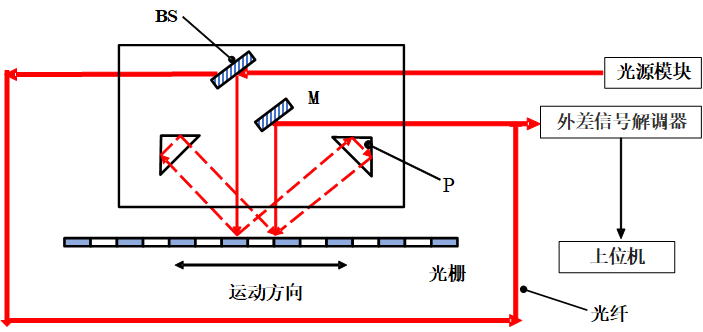
\includegraphics[width=1\textwidth]{3-fig/光栅位移测量系统光路图.png}
  \caption{光栅位移测量系统光路图}
  \label{fig:光栅位移测量系统光路图}
\end{figure}

在此对其进行多普勒频移分析,由上文可知,当激光垂直入射到光栅,光源模块作为发射源,反射光栅作为接收物体,以速度$\upsilon $沿着光栅平面运动,此时各级次的衍射光会产生多普勒频移$\Delta f$:
\begin{equation}
  \Delta f=\frac{k v}{D}
\end{equation}

光源模块的激光光束第一次在反射光栅发生衍射时,+1级衍射光和-1级衍射光分别会产生频移:
\begin{equation}
  \Delta f_{1}=\frac{v}{D}
\end{equation}
\begin{equation}
  \Delta f_{-1}=-\frac{v}{D}
\end{equation}

此时在角锥棱镜的作用下,衍射光束原路返回再次入射到光栅表面,此时会再次产生多普勒频移:
\begin{equation}
  \Delta f_{(1,1)}=\frac{v}{D}
\end{equation}
\begin{equation}
  \Delta f_{(-1,-1)}=-\frac{v}{D}
\end{equation}

会和后的光束会发生拍频,其频率为:
\begin{equation}
  \left(f_{1} + \Delta f_{1}+\Delta f_{(1,1)}\right)-\left(f_{2} - \Delta f_{-1}-\Delta f_{(-1,-1)}\right)=\left(f_{1}-f_{2}\right) + 4 \frac{v}{D}
\end{equation}

上式产生的测量信号与双频激光器输出的参考信号相减即可得到包含有位移信息的多普勒频移$\Delta f$。被测光栅的位移$L$与$\Delta f$的关系可表示为:
\begin{equation}
  L=\int_{0}^{t}v d t=\int_{0}^{t} \frac{\Delta f \cdot d}{4} d t=\frac{d}{4} \int_{0}^{t} \Delta f d t=\frac{D}{4}N
\end{equation}

由上式可知,当光栅移动一个光栅栅距$D$时,在干涉信号上表现为4各个周期性的明暗变化。由此也可看出,本文所设计的光路结构实现了光学四倍频,提高了系统的分辨率。

\subsection{光源模块的设计}
本实验的光源模块输出的是两束相互垂直具有频差的线偏振光。其实现原理如图\ref{fig:光源模块设计图}。激光器发出的光束经过1/4波片得到线偏振光,垂直入射到偏振分光镜PBS上,被分为两束光,其中P光完全透过,经过声光移频器改变频率;S光被反射进入另外一个声光移频器,两者的频差可以进行调节。之后再经过直角反射镜调节方向,光束位移调节器确定光束仰角,1/2波片改变偏振方向,汇合在偏振分光镜处。最后经过准直扩束镜,耦合进光纤输出。
\begin{figure}[H]
  \centering
  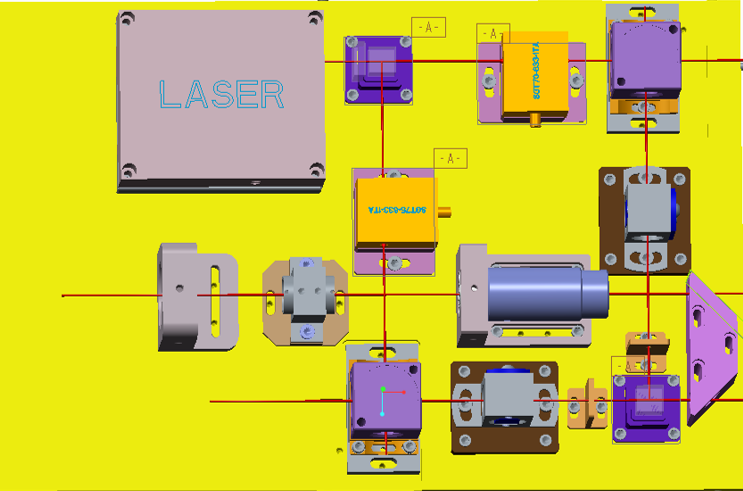
\includegraphics[width=1\textwidth]{3-fig//光源模块设计图.png}
  \caption{光源模块设计图}
  \label{fig:光源模块设计图}
\end{figure}
\subsubsection{声光移频器}
在外差干涉测量装置中,最重要的就是输出频率不同的两束光,也就是在参考光和测量光之间引入差频,才能将高频的信息转移到低频的拍频中去。目前常用的移频方式主要分为两类,一种是机械式调制频率,但采用机械式调制可能在调制过程中产生机械震荡,引入误差,现使用较少。另一种则主要采用电子式调制频率,按照调制的方法可以分为:基于塞曼效应(Zeeman effect)、声光调制器(Acousto-Optical Modulator,AOM)、电光晶体调制器(Electro-Optical Modulator,EOM)三种。

塞曼效应\cite{thalau2006magnetic,preston1898radiation}是1896年由荷兰物理学家Pieter Zeeman提出的,他发现当光源置于外加磁场中时,原来的谱线会分裂成几条谱线,而分裂出来的谱线分量是偏振的,且分裂的数量随能级的类别而变化。随后Hendrik Antoon Lorentz在理论上解释了谱线分裂的原因\cite{sargent1967theory}。根据塞曼效应,可以通过控制磁场来调节两个偏振激光器的频率差。基于此原理,可以制造出双频激光器\cite{rong2003frequency}。然而,塞曼激光器由于价格高、光源强度弱而没有被选作外差光源。

电光晶体调制器\cite{李洪祚2008电光调制器}是利用一些电光晶体的电光效应制成的调制器,如铌酸锂晶体(LiNbO3)、砷化镓晶体(GaAs)和钽酸锂晶体(LiTaO3)。电光效应是指当对电光晶体施加电压时,电光晶体的折射率会发生变化,从而导致光波通过晶体的特性发生变化,实现调制光信号的相位、幅度、强度和偏振态。电光晶体调制器结构简单,工作稳定,但存在插入损耗,并且由于热不均匀等原因,电光晶体调制器经常发生位移,影响调制质量。

声光调制器\cite{尚建华2012基于双声光移频器的外差式激光多普勒测振计,郭力仁2015声光移频器对微多普勒效应探测的影响研究}使用声光相互作用来获得光的频移。原始信号在声光移频器的作用下新增一个移频信号。此移频信号的大小等于施加在声光移频器上的功率信号的频率。当输出光选择正一级衍射光时,其频率为原始激光频率与电信号频率之和;当输出光选择负一级衍射光时,其频率为原始激光频率与电信号频率之差。这样就可以控制输入信号的频率来调节输出光的频率,或者可以保持驱动频率不变,以不同的衍射级作为输出。声光调制的工作原理如图\ref{fig:声光调制器原理}所示:
\begin{figure}[H]
  \centering
  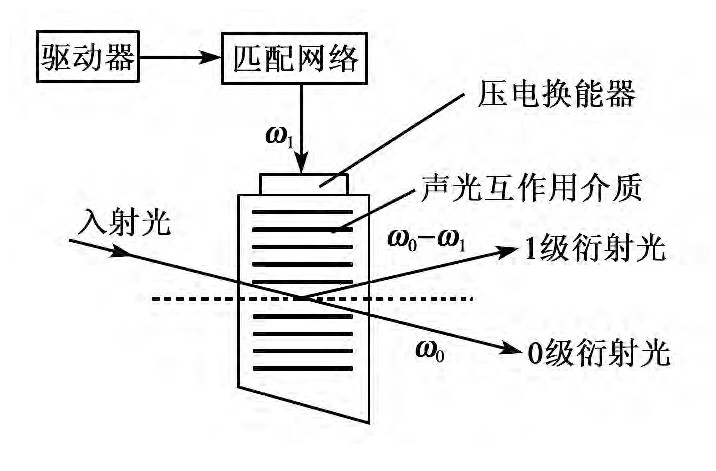
\includegraphics[width=0.7\textwidth]{3-fig//声光调制器原理.jpg}
  \caption{声光调制器原理}
  \label{fig:声光调制器原理}
\end{figure}
当驱动信号通过压电换能器时,会产生一个超声波场,此时声波在介质中的传播会在超声波场的作用下发生弹性变形。当光波通过声光移频器时,会与驱动信号产生的超声波发生相互作用,产生衍射现象。当超声波和光波的入射角满足一定条件时,各级衍射光会相互干涉和抵消。此时,光场中只剩下0级和±1级衍射光。这种衍射现象称为布拉格衍射。

在满足布拉格衍射的条件下,通过声光调制器的理论1级衍射光强为:
\begin{equation}
  I_{1}=I_{\mathrm{i}} \sin ^{2}\left(\frac{v}{2}\right)
\end{equation}
其中$I_{\mathrm{i}}$表示入射光光强,$\upsilon $表示光波穿过超声场时的附加相位延迟。
\begin{equation}
  v=\frac{2 \pi}{\lambda_{0}} \Delta n L=2 \frac{\pi}{\sqrt{2} \lambda_{0}} \sqrt{\frac{L}{H} M P_{\mathrm{A}}} =2 \frac{\pi}{\sqrt{2} \lambda_{0}} \sqrt{\frac{L}{H} \frac{P^{2} n^{6}}{\rho v_{\mathrm{s}}^{3}} P_{\mathrm{A}}}
\end{equation}
其中M为声光介质的品质因素,P为声光系数,$\rho $为声光晶体的密度,n为声光晶体的折射率,$ \lambda_{0}$为光的波长,$v_{\mathrm{s}}$为声速,$P_{\mathrm{A}}$为声波功率,L、H为换能器的长和宽。

代入可得:
\begin{equation}
  I_{1}=I_{\mathrm{i}} \sin ^{2}\left(\sqrt{\frac{L \pi^{2} P^{2} n^{6}}{2 H \rho \lambda_{\mathrm{o}}^{2} v_{\mathrm{s}}^{3}} P_{\mathrm{A}}}\right) \approx I_{\mathrm{i}}\left(\frac{L \pi^{2} P^{2} n^{6}}{H \rho \lambda_{\mathrm{o}}^{2} v_{\mathrm{s}}^{3}}\right) P_{\mathrm{A}}
\end{equation}

与电光晶体调制器相比,声光调制器具有诸多优点,比如更低的驱动功率和更好的温度稳定性;与机械调制相比,声光调制器体积更小,重量更轻,输出波形更好。因此在本文的光源模块设计中,采用声光调制器来进行移频。

\subsubsection{其他光学元件}
本文设计的光源中使用的其他光学元件有反射镜、1/4波片、1/2波片、偏振分光棱镜(PBS)、光束位移调节器、准直扩束镜、光束角度调节器。为了保证原始信号的质量,避免光学元件的光能损失和杂散光,需要仔细选择合适的光学元件。具体的光学元件如表\ref{tab:光源模块需要用到的光学元器件}所示。
\begin{figure}[htb]
  \centering
  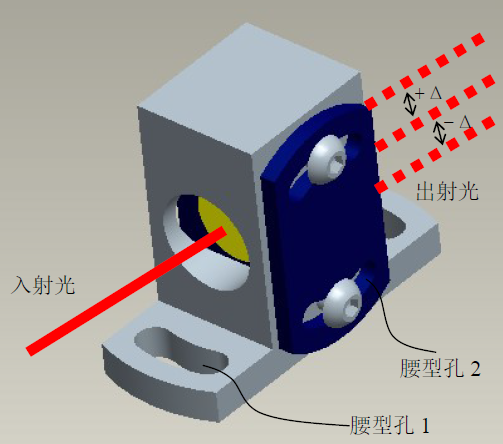
\includegraphics[width=5cm]{3-fig//光束位移调节器.png}
  \caption{光束位移调节器}
  \label{fig:光束位移调节器}
\end{figure}
\begin{figure}[htb]
  \centering
  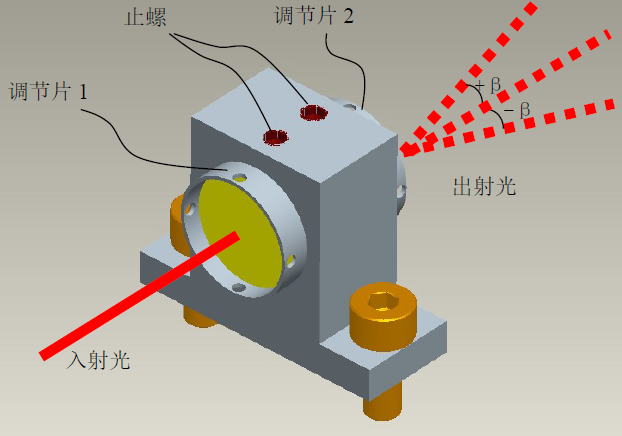
\includegraphics[width=5cm]{3-fig//光束角度调节器.png}
  \caption{光束角度调节器}
  \label{fig:光束角度调节器}
\end{figure}

\begin{table}[H]
  \centering
  \caption{光源模块需要用到的光学元器件}
  \label{tab:光源模块需要用到的光学元器件}
  \begin{tabular}{cccc}
    \hline
    元件              & 尺寸/mm  & 数量 \\ \hline
    单频激光器        & 10×20×5  & 1    \\ \hline
    声光移频器        & 10×20×5  & 2    \\ \hline
    1/4波片           &          & 1    \\ \hline
    真零级增透1/2波片 &          & 2    \\ \hline
    偏振分光镜        & 10×10×10 & 2    \\ \hline
    反射镜            & 25×25×25 & 2    \\ \hline
    光束位移调节器    & 40×30×20 & 2    \\ \hline
    光束角度调节器    & 32×25×19 & 1    \\ \hline
    准直扩束镜        &          & 1    \\ \hline
  \end{tabular}
\end{table}


\subsection{读数头模块的设计}
在进行读数头模块设计时首先需要考虑所使用的光栅类型,通常情况下选择反射光栅作为测量光栅,又可细分为单光栅系统和双光栅系统。双光栅位移测量系统在测量过程中对双光栅的相对位置要求较高,本文所设计光路结构采用单反射光栅进行测量。

\subsubsection{光学倍频}
光栅位移测量系统的基本原理是利用偏振分光棱镜作为分光元件,将两束光分别入射到反射光栅上,在光栅进行位移时,反射回的光束携带位移信息,再经过一系列光学元件后汇合,发生干涉,再通过后续信号处理解调出位移信息。

图\ref{fig:基本的光栅位移测量系统}是最常见的单光栅位移测量系统。
\begin{figure}[htb]
  \centering
  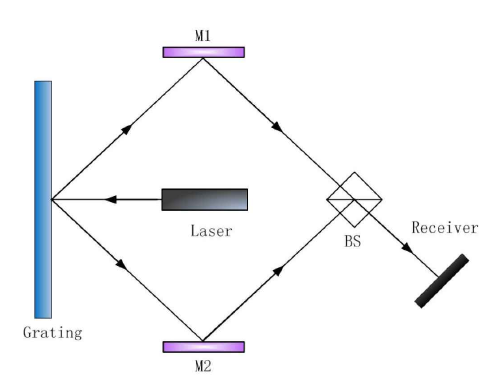
\includegraphics[width=8cm]{3-fig//最基本的光栅位移测量系统.png}
  \caption{基本的光栅位移测量系统}
  \label{fig:基本的光栅位移测量系统}
\end{figure}

单频激光器发射出的光束垂直入射到光栅上发生一次衍射,得到的两束携带位移信息的光束通过反射镜和分光镜在光电探测器处汇合,得到含有位移信息的拍频信号。

本文根据上述光路设计原理,对基本的单光栅位移测量系统光路进行改进,设计了一种新的基于二次衍射的单光栅位移测量光路。所设计的光学系统如图\ref{fig:读数头模块}所示。激光器发出的激光射向反射光栅,一次衍射光通过角锥棱镜反射回光栅进行二次衍射,将二次衍射光作为测量信号。这种光学系统的优点是它使用较少的光学元件来达到光学倍频的效果,能够将读数头模块进行集成小型化。

\begin{figure}[htb]
  \centering
  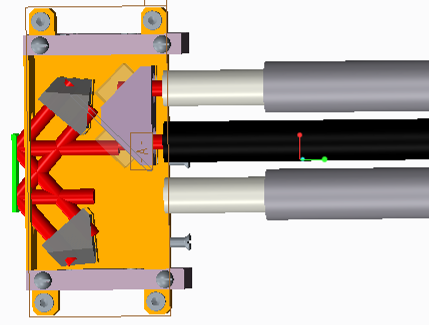
\includegraphics[width=0.5\textwidth]{3-fig//读数头模块.png}
  \caption{读数头模块}
  \label{fig:读数头模块}
\end{figure}

\subsubsection{角锥棱镜}
常用的反射镜有平面反射镜、直角棱镜反射镜、角锥棱镜反射镜。

平面反射镜结构简单,对横向移动不敏感,但是当平面镜有$\theta $的角度偏转时,反射光光线就会有$2\theta $的角度偏转,这个误差会对光路结构有很大的影响,所以不使用。

直角棱镜反射镜如图\ref{fig:直角棱镜}所示,三个角分别为45°、45°、90°。两个斜面都可以作为反射面,两个直角边也可以作为反射面。主要用于光路的转向,结构简单,加工成本低,但使用时只有一个方向自对准,另一个方向不能控制方向。
\begin{figure}[H]
  \centering
  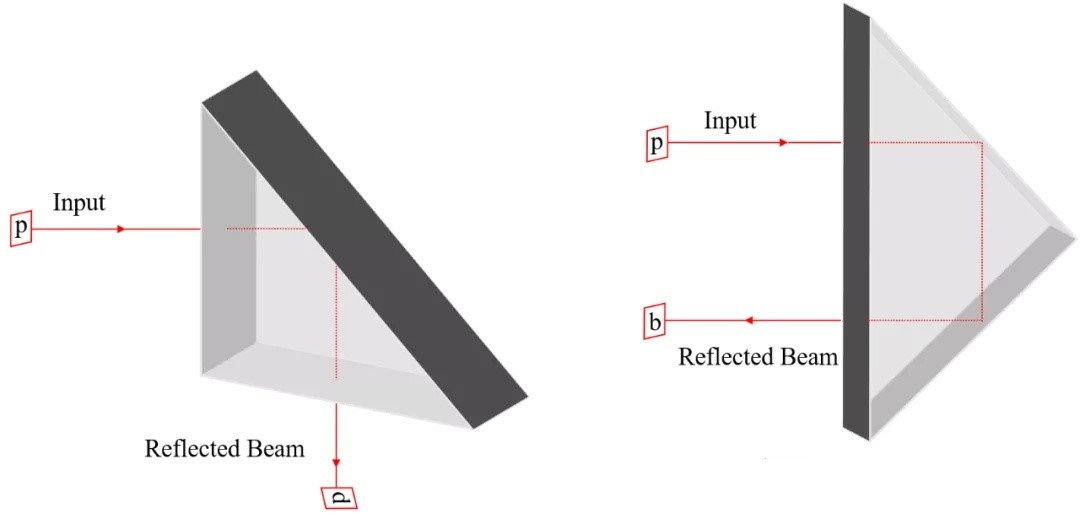
\includegraphics[width=0.8\textwidth]{3-fig//直角棱镜.jpg}
  \caption{直角棱镜}
  \label{fig:直角棱镜}
\end{figure}

角锥棱镜由三个相互垂直的直角面组成,入射光在三个直角面上形成全反射,返回原路。角锥棱镜对光的入射角不敏感,棱镜绕任意轴旋转不影响出射光束的方向,因此使用角锥棱镜可以大大降低安装要求。
\begin{figure}[H]
  \centering
  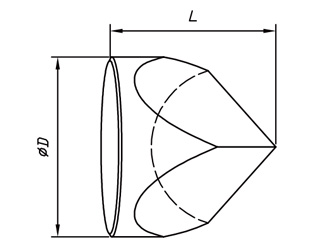
\includegraphics[width=0.5\textwidth]{3-fig//角锥棱镜.jpg}
  \caption{角锥棱镜}
  \label{fig:角锥棱镜}
\end{figure}

\section{光路系统的琼斯矩阵推导}
\subsection{偏振光学理论}
在光栅位移测量系统中,所设计光路为偏振光路,光的偏振态可以用多种方式表示。这里用琼斯矩阵来表示偏振光的变化和偏振器件的特性。由于可以忽略具体的中间物理过程,因此光路分析可以变得清晰和简单。本节将介绍偏振光和偏振器件的琼斯矩阵。
\subsubsection{偏振光的琼斯矩阵}
当偏振光沿Z轴进行传播时,偏振光可以用沿着x轴和y轴的线偏振光的叠加来表示:
\begin{equation}
  \boldsymbol{E}=E_{x} \boldsymbol{x}_{\theta}+E_{y} \boldsymbol{y}_{\theta}=a_{1} \boldsymbol{x}_{\theta} \exp \left[i\left(\alpha_{1}-\omega t\right)\right]+a_{2} \boldsymbol{y}_{0} \exp \left[i\left(\alpha_{2}-\omega t\right)\right]
\end{equation}

\begin{figure}[H]
  \centering
  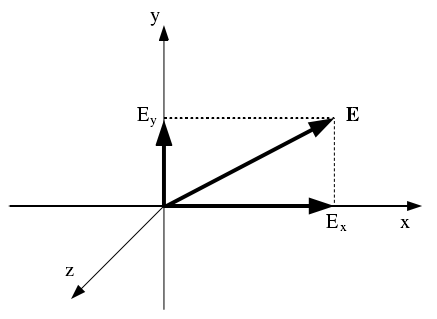
\includegraphics[width=0.5\textwidth]{3-fig//偏振光的表示.png}
  \caption{光矢量在x,y轴的分量表示}
  \label{fig:光矢量在x,y轴的分量表示}
\end{figure}

偏振光用光矢量分量所构成的矩阵表示,这一矩阵即为琼斯矩阵。
\begin{equation}
  \boldsymbol{E}=\left[\begin{array}{c}
      E_{x} \\
      E_{y}
    \end{array}\right]=\left[\begin{array}{l}
      a_{1} \exp \left(i \alpha_{1}\right) \\
      a_{2} \exp \left(i \alpha_{2}\right)
    \end{array}\right]
\end{equation}

将琼斯矢量进行归一化,提取出公共因子得到:
\begin{equation}
  \boldsymbol{E}=\frac{a_{1} \exp \left(i \alpha_{1}\right)}{\sqrt{a_{1}^{2}+a_{2}^{2}}}\left[\frac{1}{a_{2}} \exp \left[i\left(\alpha_{2}-\alpha_{1}\right)\right]\right]=\frac{a_{1} \exp \left(i \alpha_{1}\right)}{\sqrt{a_{1}^{2}+a_{2}^{2}}}\left[\begin{array}{c}
      1 \\
      a \exp (i \delta)
    \end{array}\right]
\end{equation}
其中$a=\frac{a_{2}}{a_{1}}$为两个线偏振光的振幅比,$ \delta=\alpha_{2}-\alpha_{1}$为相位差。略去公共因子,归一化后的琼斯矢量为:
\begin{equation}
  \boldsymbol{E}=\frac{a_{1}}{\sqrt{a_{1}^{2}+a_{2}^{2}}}\left[\begin{array}{c}
      1 \\
      a \exp (i \delta)
    \end{array}\right]
\end{equation}

通过上述公式,可以算出常见偏振态的琼斯矢量,如表\ref{tab:常见偏振态的琼斯矩阵}所示。
\begin{table}[H]
  \centering
  \caption{常见偏振态的琼斯矩阵}
  \label{tab:常见偏振态的琼斯矩阵}
  \begin{tabular}{cc}
    \hline
    偏振态                     & 琼斯矩阵                                                        \\ \hline
    光矢量沿X轴                & $\left[\begin{array}{c}1 \\ 0\end{array}\right]$                   \\ \hline
    光矢量沿Y轴                & $\left[\begin{array}{c}0 \\ 1\end{array}\right]$                   \\ \hline
    光矢量与X轴呈±45°          & $\frac{1}{\sqrt{2}}\left[\begin{array}{c}1 \\ \pm 1\end{array}\right]$ \\ \hline
    光矢量与X轴呈$\pm \theta $ & $\left[\begin{array}{c}\cos \theta \\ \pm \sin \theta\end{array}\right]$                   \\ \hline
  \end{tabular}
\end{table}

\subsubsection{偏振器件的琼斯矩阵}
当偏振光经过偏振器件时,一般它的偏振状态都会发生改变。假设入射光的偏振态用$\boldsymbol{E}_{i}=\left[\begin{array}{l}A_{1} \\ B_{1}\end{array}\right]$表示,出射光的偏振态用$\boldsymbol{E}_{t}=\left[\begin{array}{l}A_{2} \\ B_{2}\end{array}\right]$表示。偏振器件$\boldsymbol{G}$在中间起着变换作用,假设这种变换是线性的,那么
\begin{equation}
  \begin{aligned}
     & A_{2}=g_{11} A_{1}+g_{12} B_{1} \\
     & B_{2}=g_{21} A_{1}+g_{22} B_{1}
  \end{aligned}
\end{equation}
其中,$g_{11}$,$g_{12}$,$g_{21}$,$g_{22}$是常数。把上式写成矩阵形式即为:
\begin{equation}
  \left[\begin{array}{l}
      \mathrm{A}_{2} \\
      \mathrm{~B}_{2}
    \end{array}\right]=\left[\begin{array}{ll}
      \mathrm{g}_{11}  & \mathrm{~g}_{12} \\
      \mathrm{~g}_{21} & \mathrm{~g}_{22}
    \end{array}\right]\left[\begin{array}{l}
      \mathrm{A}_{1} \\
      \mathrm{~B}_{2}
    \end{array}\right]
\end{equation}
其中,$\boldsymbol{G}=\left[\begin{array}{ll}g_{11} & g_{12} \\ g_{21} & g_{22}\end{array}\right]$代表偏振器件的琼斯矩阵。常见的偏振器件的琼斯矩阵如表\ref{tab:常见偏振器件的琼斯矩阵}所示。
\begin{table}[htb]
  \centering
  \caption{常见偏振器件的琼斯矩阵}
  \label{tab:常见偏振器件的琼斯矩阵}
  \begin{tabular}{ccc}
    \multicolumn{2}{c}{偏振器件}                 & 琼斯矩阵                                                                                       \\ \hline
    \multirow{4}{*}{线偏振器}                    & 光矢量沿X轴                & $\left[\begin{array}{cc}1 & 0 \\ 0 & 0\end{array}\right]$                     \\
                                                 & 光矢量沿Y轴                & $\left[\begin{array}{cc}0 & 0 \\ 0 & 1\end{array}\right]$                     \\
                                                 & 光矢量与X轴呈±45°          & $\frac{1}{\sqrt{2}}\left[\begin{array}{cc}1 & \pm 1 \\ \pm 1 & 1\end{array}\right]$   \\
                                                 & 光矢量与X轴呈$\pm \theta $ & $\left[\begin{array}{cc}\cos ^{2} \theta & \frac{1}{2} \sin 2 \theta \\ \frac{1}{2} \sin 2 \theta & \sin ^{2} \theta\end{array}\right]$                     \\ \hline
    \multicolumn{1}{l}{\multirow{3}{*}{1/4波片}} & 快轴在X方向                & $\left[\begin{array}{cc}1 & 0 \\ 0 & i\end{array}\right]$                    \\
    \multicolumn{1}{l}{}                         & 快轴在Y方向                & $\left[\begin{array}{cc}1 & 0 \\ 0 & -i\end{array}\right]$                    \\
    \multicolumn{1}{l}{}                         & 快轴与X轴夹角±45°          & $\frac{1}{\sqrt{2}}\left[\begin{array}{cc}1 & \mp i \\  \mp i & 1\end{array}\right] $ \\ \hline
  \end{tabular}
\end{table}

\subsection{琼斯矩阵分析}
光源模块发出的激光可以表示为:
\begin{equation}
  E_{0}=\left[\begin{array}{l}
      1 \\
      0
    \end{array}\right] \exp \left(i \omega_{1} t\right)+\left[\begin{array}{l}
      0 \\
      1
    \end{array}\right] \exp \left(i \omega_{2} t\right)
\end{equation}
其中$\omega_{1}$和$\omega_{2}$分别表示两个不同频率分量的角频率。
\begin{figure}[H]
  \centering
  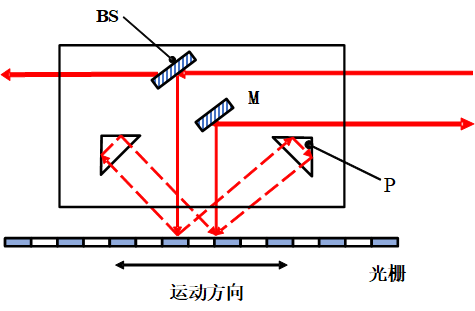
\includegraphics[width=0.5\textwidth]{3-fig//系统光路图.png}
  \caption{系统光路图}
  \label{fig:系统光路图}
\end{figure}

参考信号透过分光镜BS,再经过偏振片P,由光纤送入信号接收器。接收到的电场表达式为:
\begin{equation}
  E_{r}=\mathrm{P}(\pi / 4) \cdot \mathrm{BS}_{\mathrm{T}} \cdot E_{0}
\end{equation}

反射光束垂直入射到光栅表面,再经过角锥棱镜进行反射,有一个角锥棱镜会进行镀膜,反射的光束再次入射到光栅表面,垂直出射至反射镜汇合,由光纤送入信号接收器2。光栅的琼斯矩阵为:
\begin{equation}
  \mathrm{G}(\theta)=\mathrm{G}(-\theta)=\left[\begin{array}{cc}
      -\sqrt{\eta_{\rho}(\theta)} & 0                       \\
      0                           & \sqrt{\eta_{s}(\theta)}
    \end{array}\right]
\end{equation}
其中$\eta_{\rho}(\theta)$和$\eta_{s}(\theta)$分别表示光栅对于p光和s光的振幅反射系数。

接收到的电场表达式为:
\begin{equation}
  \begin{aligned}
    E_{t}= & \left[  \mathrm{M}  \cdot\mathrm{G}(\theta)\cdot \mathrm{HWP}(\pi / 4) \cdot  \mathrm{M2} \cdot\mathrm{G}(\theta) \exp \left(i k l_{+1}+i \phi_{+1}\right)\right.                   \\
           & \left.+\mathrm{M} \cdot \mathrm{G}(-\theta) \cdot \mathrm{Ml} \cdot \mathrm{G}(-\theta) \exp \left(i k l_{-1}+i \phi_{-1}\right) \right] \cdot \mathrm{BS}_{\mathrm{R}} \cdot E_{0}
  \end{aligned}
\end{equation}
其中$k=2 \pi n / \lambda$为空气中波矢量的表达式,$l_{+1}$和$l_{-1}$分别表示两种不同偏振态在非共光程光路下所经过的路径长度,$\phi_{+1}$和$\phi_{-1}$表示相位变化。根据上文分析的多普勒频移理论,当光栅运动位移$\Delta s$后,$\phi_{+1}$和$\phi_{-1}$可分别表示为:
\begin{equation}
  \phi_{\pm 1}=\pm 4 \pi \Delta s / D
\end{equation}
其中D为光栅常数。将上式代入可得:
\begin{equation}
  E_{r}=\frac{1}{2 \sqrt{2}}\left[\begin{array}{ll}
      1 & 1 \\
      1 & 1
    \end{array}\right] \cdot\left[\begin{array}{l}
      \exp \left(i \omega_{1} t\right) \\
      \exp \left(i \omega_{2} t\right)
    \end{array}\right]
\end{equation}
\begin{equation}
  E_{t} \propto \left[\exp \left(i \omega_{1} t+i k l_{-1}+i \phi_{-1}\right)+\exp \left(i \omega_{2} t+i k l_{+1}+i \phi_{+1}\right)\right]
\end{equation}
由于光强信号是电场强度与其共轭的成绩,相乘后可以得到:
\begin{equation}
  I_{r} \propto \cos \left[\left(\omega_{1}-\omega_{2}\right) t\right]
\end{equation}
\begin{equation}
  I_{t} \propto  \cos \left[\left(\omega_{1}-\omega_{2}\right) t+k\left(l_{-1}-l_{+1}\right)+\left(\phi_{-1}-\phi_{+1}\right)\right]
\end{equation}

参考信号和测量信号通过光电探测器转换为电子信号之后,送入外差信号解调器中,测得两者之间的相位差:
\begin{equation}
  \phi_{m}=k\left(l_{-1}-l_{+1}\right)+\left(\phi_{-1}-\phi_{+1}\right)=\phi_{non}+\phi_{mov}
\end{equation}
其中,$\phi_{non}$为非共光程光路所引起的相位变化,$\phi_{mov}$为光栅运动引起的相位变化。$\phi_{non}$在这里视为常数,由此得到被测位移与测量相位之间的关系为:
\begin{equation}
  s=\frac{\phi_{m}}{4 \pi} \cdot d
\end{equation}

\section{本章小结}
本章首先介绍了一下光路系统的设计原则,之后的设计也大多遵循。然后给出了外差式光栅位移测量系统的整体设计方案,主要分为两大部分,光源模块的设计和读数头模块的设计。在光源模块的设计中介绍了外差激光的实现原理,分析了声光调制器的原理和选择方案,同时对其他光学元件进行选择。在读数头模块设计中,基于原有的衍射方案,提出了二次衍射测量的方法,对测量原理进行了推导,对器件进行选型。最后通过偏振光学理论对光路进行分析推导,介绍了偏振光和偏振器件的琼斯矩阵,推导了测量位移和相位之间的关系。


\chapter{光栅位移测量系统实验及其误差分析}
\section{光路调试与平台安装}
在进行光栅位移测量系统的搭建时,主要按照以下顺序进行:

(1)根据光源模块的各个结构,将激光器固定好,调整偏振分光棱镜的位置,使经过偏振分光棱镜后的透射光束能够射入声光移频器,再经过反射镜后,调整光束位置调节器,使得出射光束能够以较大光斑透过小孔汇合在偏振分光棱镜处。同样经过偏振分光棱镜后的反射光束经过调整与透射光束汇合。在出射处,通过调整光纤耦合器的角度,使得激光光束能以最大光强射入光纤,同时在光纤的另一端放置光功率计,通过观察输出功率的变化来判断是否达到最大光强,当出现极大值时,说明光源模块调试成功。

(2)根据读数头模块的各个结构,调整光纤的入射角度,使得经过光栅衍射的光束能以合适的角度打到角锥棱镜上,同时角锥棱镜反射回的光束能够顺利进行二次衍射,通过反射镜射出。

(3)运动台部分,将运动台固定在基座上,利用紫外胶点胶的方式将光栅固定在运动台上,调整读数头位置,使得读数头与运动台平行。

(4)电路解调部分,使用光纤耦合器将光束输入到三轴激光外差信号解调器上,通过观察信号曲线幅值来判断输入光的强度,通过调整耦合角度,使得信号能达到最大值。

光源模块实物图如图\ref{fig:光源模块实物图},读数头模块实物图如图\ref{fig:读数头模块实物图},整个系统实物图如图\ref{fig:系统整体实物图}。
\begin{figure}[H]
  \centering
  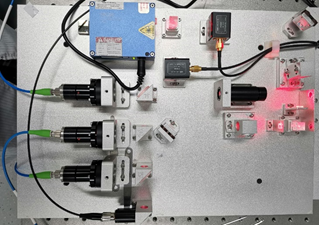
\includegraphics[width=0.5\textwidth]{4-fig//光源模块实物图.png}
  \caption{光源模块实物图}
  \label{fig:光源模块实物图}
\end{figure}
\begin{figure}[H]
  \centering
  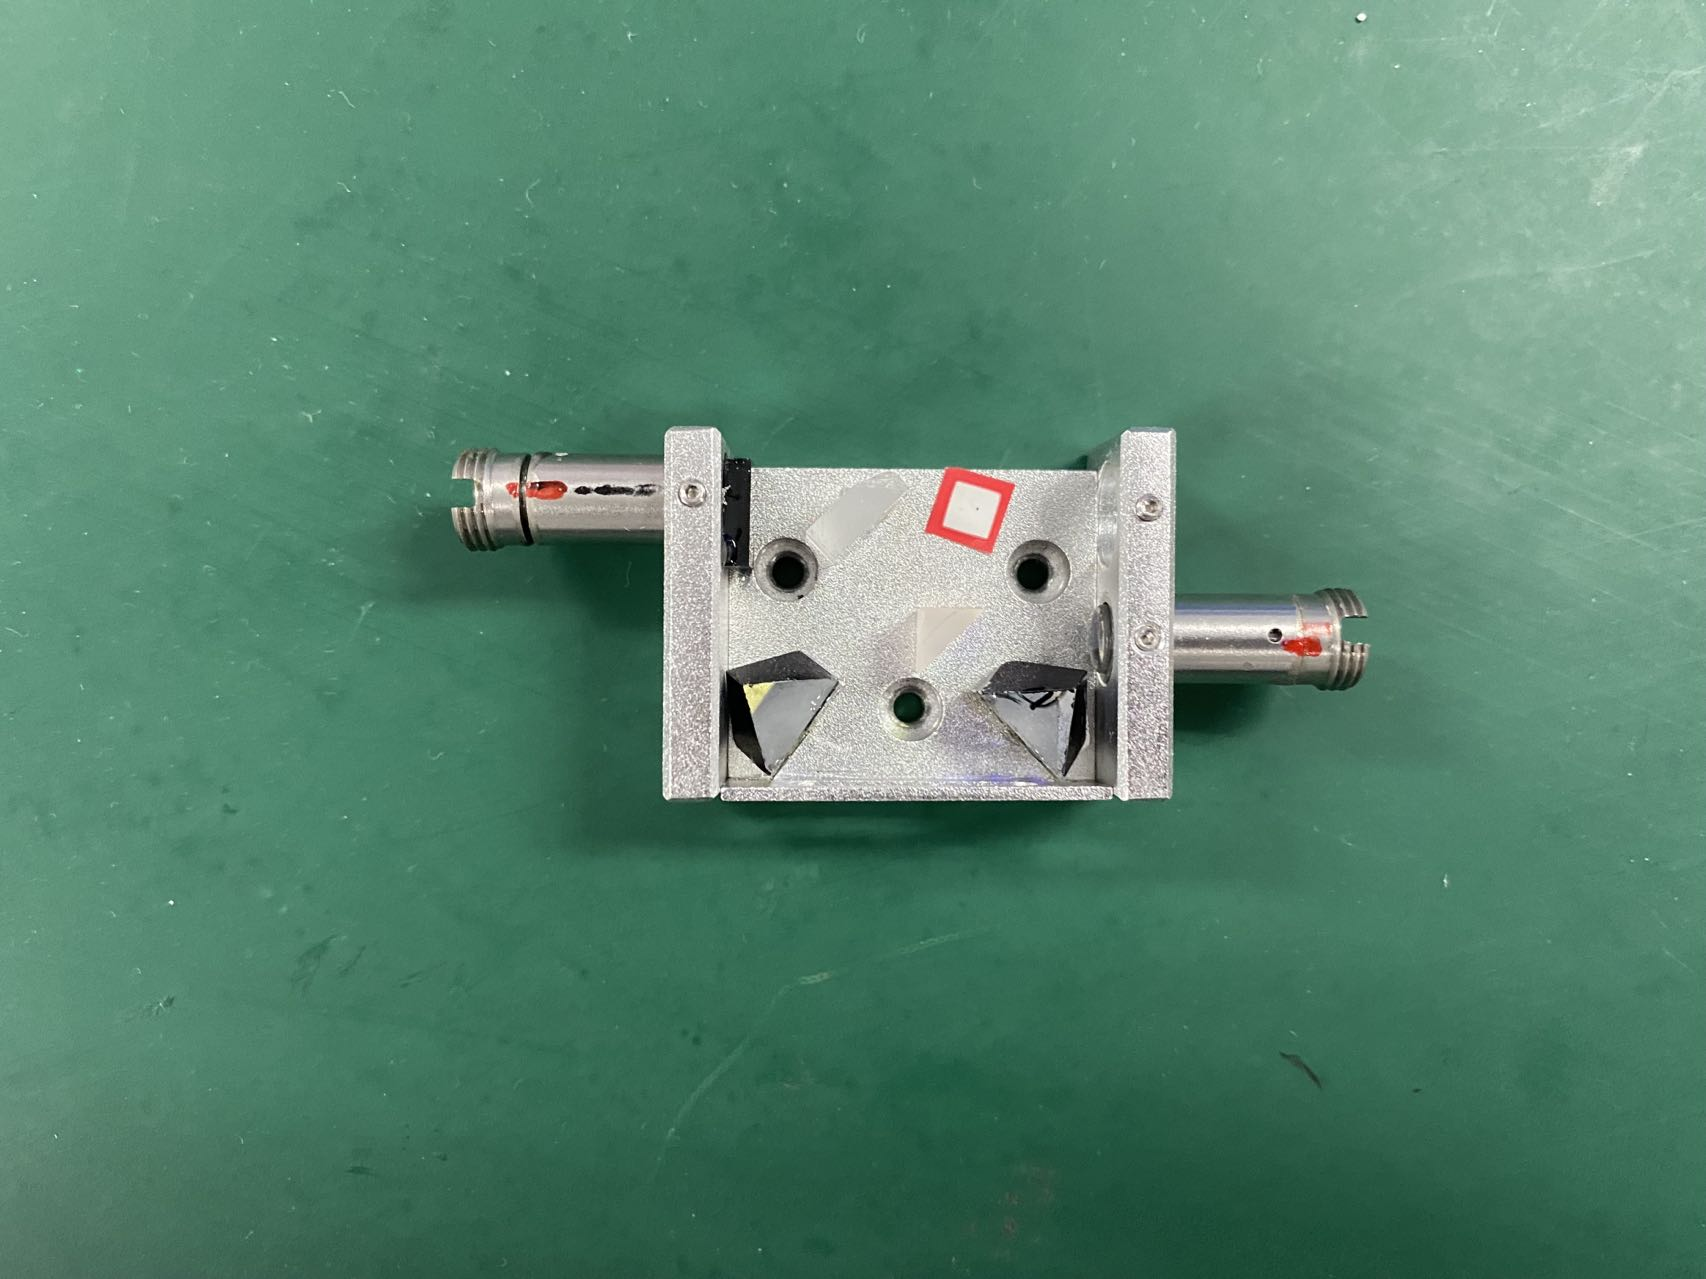
\includegraphics[width=0.5\textwidth]{4-fig//读数头模块实物图.jpg}
  \caption{读数头模块实物图}
  \label{fig:读数头模块实物图}
\end{figure}
\begin{figure}[H]
  \centering
  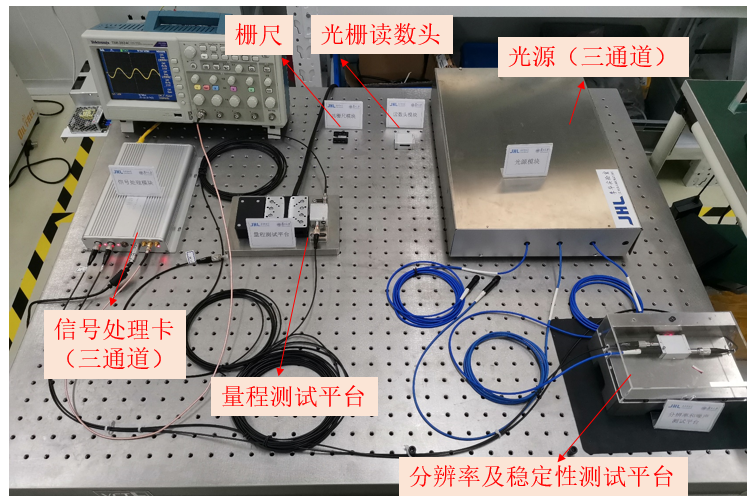
\includegraphics[width=1\textwidth]{4-fig//整体实验装置图.png}
  \caption{系统整体实物图}
  \label{fig:系统整体实物图}
\end{figure}

\section{性能测试和结果}
本节将对所设计的光栅位移测量系统进行实验测试,分析其在不同实验条件下的表现。主要分为两大部分,第一部分是行程测量,通过改变行进距离,行进步距等条件来进行综合测试,评估系统的运动性能。第二部分是稳定性测量,通过分析在静止状态下的光栅位移波动来评估系统的稳定性,反过来也可通过不断优化实验条件,来使系统的稳定性达到最好,避免外界环境干扰因素。

本文所采用的驱控器如图\ref{fig:驱控器接口}所示,是联合光科生产的JC-4304-X,是一款压电马达驱动的精密电动位移台。驱控器接1个M304马达或2个并联的M302压电马达,位置反馈和马达由同一DB15接口接入。驱控器通过USB转485接上位机或其他主机。由上位机向驱控器发送基本的运动参数和指令,如PID参数,运动速度,确定零位,步进距离,闭环行程,精度等,同时可以实时显示位移台的位置信息。
\begin{figure}[H]
  \centering
  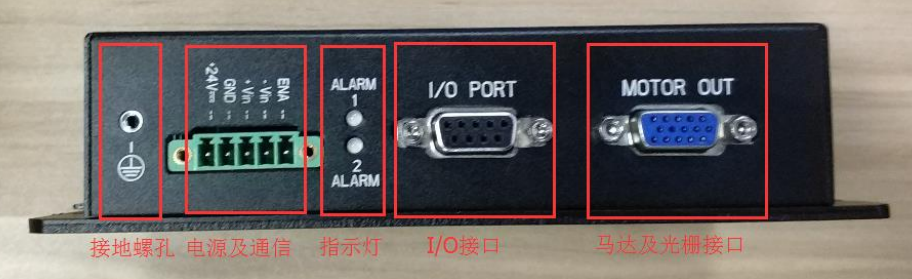
\includegraphics[width=1\textwidth]{4-fig//驱控器接口.png}
  \caption{驱控器接口}
  \label{fig:驱控器接口}
\end{figure}

软件设置界面如图\ref{fig:运动台控制软件}所示。默认位置显示单位为count,当光栅尺精度为 50nm 时,1count 对应 50nm。实验过程中,通过改变步距,停留时间,总行程等参数来评估光栅位移测量系统的性能。
\begin{figure}[H]
  \centering
  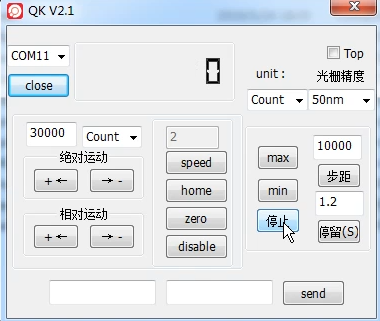
\includegraphics[width=0.7\textwidth]{4-fig//运动台控制软件.png}
  \caption{运动台控制软件}
  \label{fig:运动台控制软件}
\end{figure}

\subsection{短行程位移测试}
对于短行程位移测试,通过软件控制运动台步距为50count,100count,总行程为2500count,记录光栅的位移往返轨迹。运动间隔设置为1s。图\ref{fig:步距50行程2500运动轨迹}和图\ref{fig:步距100行程2500运动轨迹}所示为光栅位移测量系统的测试结果。

\begin{figure}[H]
  \centering
  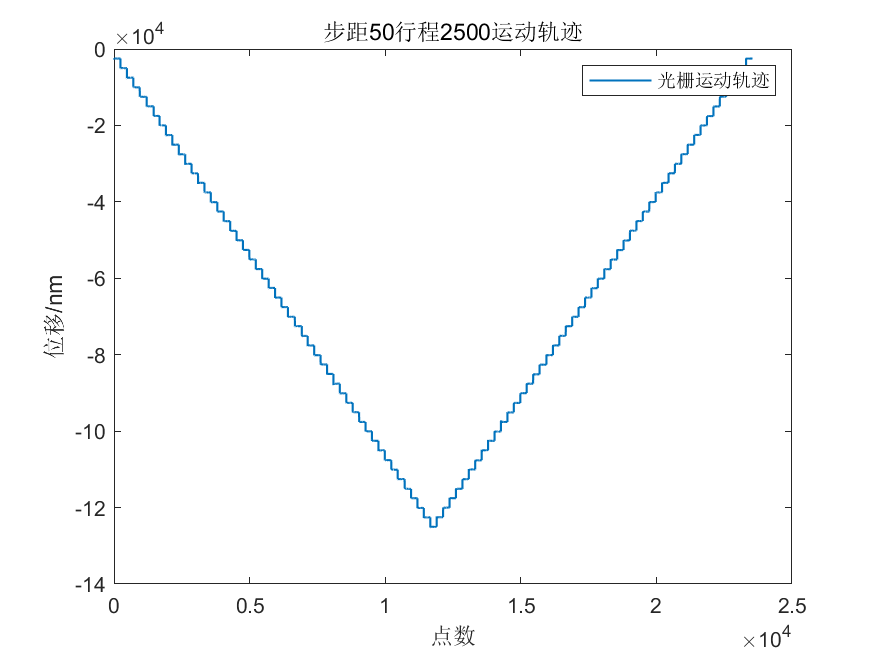
\includegraphics[width=0.8\textwidth]{4-fig//步距50行程2500运动轨迹.png}
  \caption{步距50行程2500运动轨迹}
  \label{fig:步距50行程2500运动轨迹}
\end{figure}

\begin{figure}[H]
  \centering
  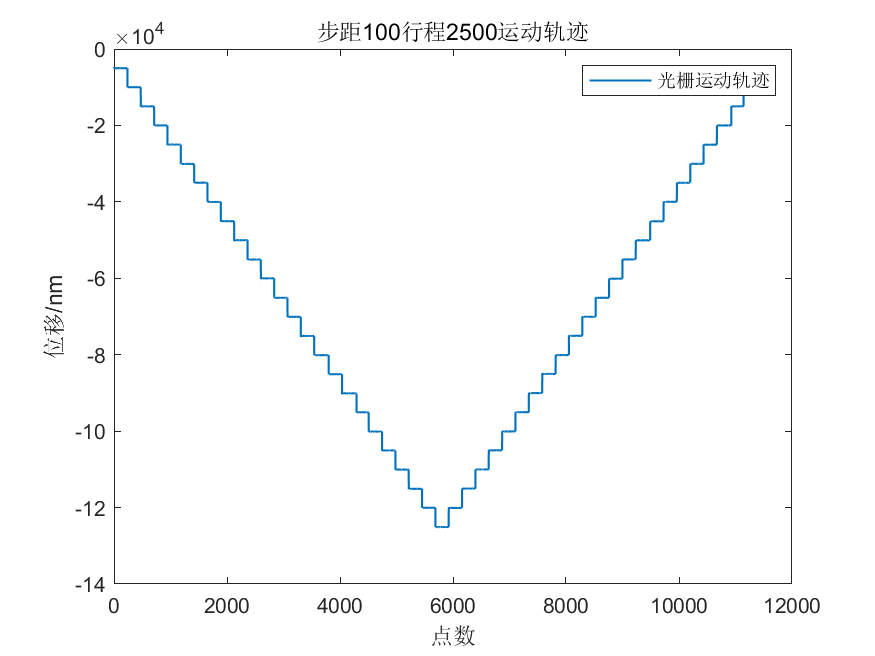
\includegraphics[width=0.8\textwidth]{4-fig//步距100行程2500运动轨迹.png}
  \caption{步距100行程2500运动轨迹}
  \label{fig:步距100行程2500运动轨迹}
\end{figure}

从图中可以看出,所设计的光栅位移测量系统能够准确的辨别每一步的步距位移大小,在图上表现出来就是阶梯状运动。在步距50,步数25步后,能够准确达到预设的终点位置,在返程中也能较好的返回起始位置。

根据重复性\cite{chassagne20072d}的定义:
\begin{equation}
  \text { Repeatabiltiy }=\left[\frac{1}{n} \sum_{i=1}^{n}\left(x_{i}^{s}-x_{i}^{e}\right)^{2}\right]^{\frac{1}{2}}
\end{equation}
其中$x_{i}^{s}$指光栅位移测量系统在初始行程中各点的位移值,$x_{i}^{e}$指返程状态下各点的位移值,$n$为运动过程中所测得数据点的个数。

利用往返运动下的各项数据,通过重复性的定义可以求得该系统的重复性为3.835nm,说明系统的重复性良好。

放大行程图,从图\ref{fig:放大行程结果}中可以看出,该系统在每一步的阶梯运动过程中的测量结果都有明显的波动,其产生原因是运动台在自身运动惯性作用下导致的位移抖动。在实际测量过程中,可以将停留时间设置稍长,等待运动台稳定后进行读数。
\begin{figure}[H]
  \centering
  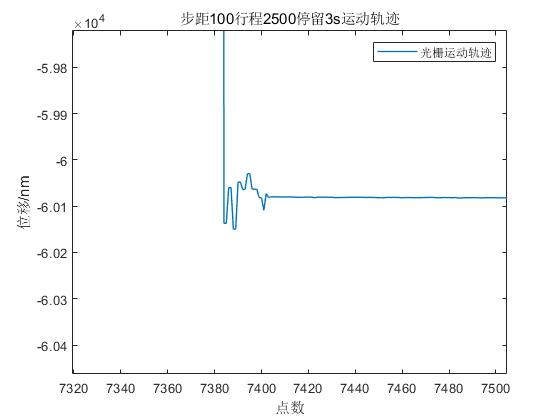
\includegraphics[width=0.8\textwidth]{4-fig//放大行程结果.jpg}
  \caption{放大行程结果}
  \label{fig:放大行程结果}
\end{figure}

\subsection{长行程位移测试}
对于长行程测试,通过软件控制运动台总行程为5000count和10000count,记录光栅往返轨迹。运动间隔设置为1s,运动步距设置为100count。并将测量结果与激光干涉仪进行对比。

如图\ref{fig:步距100行程5000运动轨迹}和\ref{fig:步距100行程10000运动轨迹}所示是位移量为5000count和10000count的长行程实验结果,从图中可以看出光栅位移曲线与干涉仪位移曲线几乎重合。

将数据采用线性回归方程拟合分析法进行分析。根据决定系数$R^{2}$,判断回归线与观测值的拟合程度。$R^{2}$最大值为1。$R^{2}$的值越接近1,回归线与观测值的拟合越好;相反,$R^{2}$的值越小,回归线与观测值的拟合越差。常用计算公式如下:
\begin{equation}
  R^{2}(y, \hat{y})=1-\frac{\sum_{i=0}^{n_{\text {samples }}-1}\left(y_{i}-\hat{y}_{i}\right)^{2}}{\sum_{i=0}^{n_{\text {samples }}-1}\left(y_{i}-\bar{y}\right)^{2}}
\end{equation}

计算出的决定系数$R^{2}$分别为0.99976和0.99975,已经非常接近1。实验结果表明,光栅位移测量系统的数据与线性回归曲线的拟合程度非常高,同时从方程中也可以看出,该系统与对比装置激光干涉仪的测量结果呈现出良好的45°线性关系。也表明所设计的光栅位移测量系统具有良好的长行程测量能力。但是,从线性方程组也可以看出,存在一个常数差异,这可能来自于一些系统误差。对于误差的分析将会放到下一小节进行分析。

\begin{figure}[H]
  \centering
  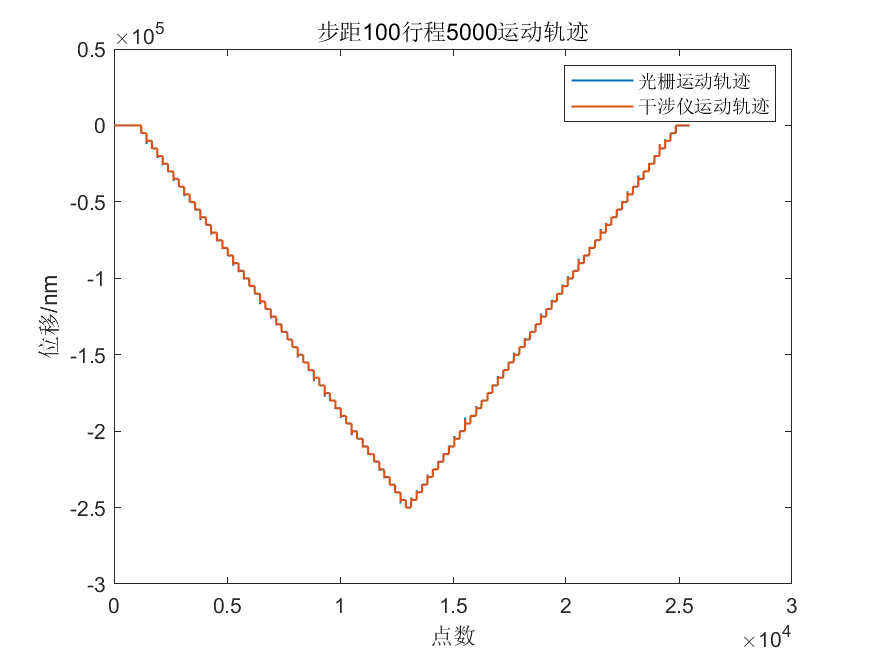
\includegraphics[width=0.8\textwidth]{4-fig//步距100行程5000运动轨迹.png}
  \caption{步距100行程5000运动轨迹}
  \label{fig:步距100行程5000运动轨迹}
\end{figure}

\begin{figure}[H]
  \centering
  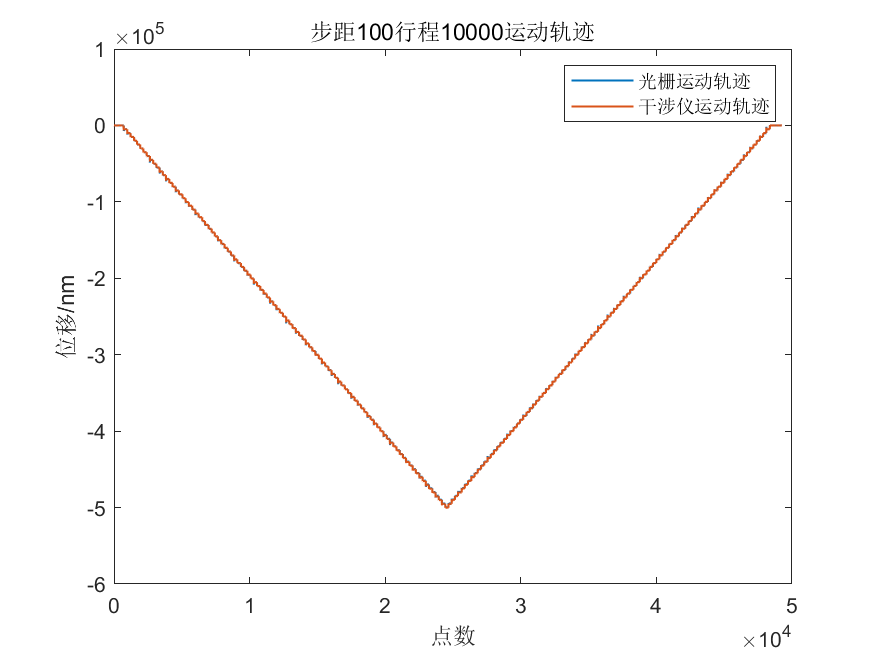
\includegraphics[width=0.8\textwidth]{4-fig//步距100行程10000运动轨迹.png}
  \caption{步距100行程10000运动轨迹}
  \label{fig:步距100行程10000运动轨迹}
\end{figure}

\begin{figure}[H]
  \centering
  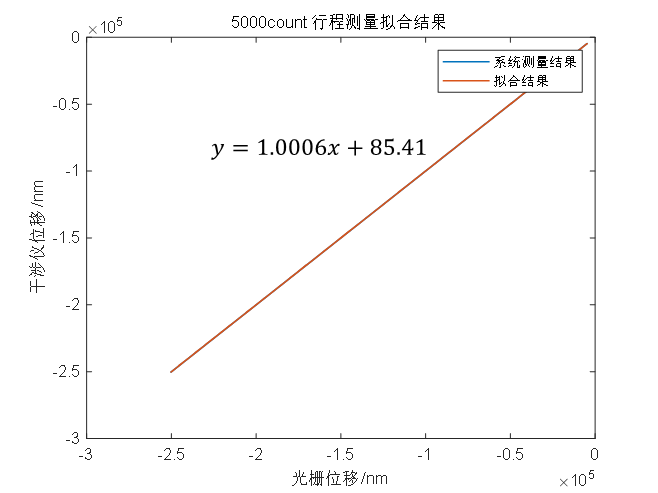
\includegraphics[width=0.8\textwidth]{4-fig//5000count拟合结果.png}
  \caption{5000count拟合结果}
  \label{fig:5000count拟合结果}
\end{figure}
\begin{figure}[H]
  \centering
  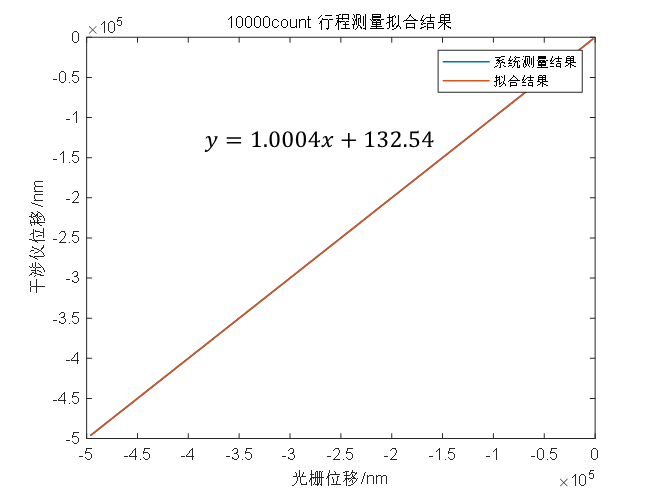
\includegraphics[width=0.8\textwidth]{4-fig//10000count拟合结果.png}
  \caption{10000count拟合结果}
  \label{fig:10000count拟合结果}
\end{figure}

\subsection{稳定性测量}
为了验证本文设计的光栅位移测量系统的稳定性,现进行稳定性测试实验。所研究的光栅位移测量系统在稳定性实验中没有使用任何补偿。实验中,平台保持稳定的时间约为3分钟,并记录了所研究的光栅位移测量系统在此期间的位移变化。

实验结果如图\ref{fig:静止状态下的稳定性}所示。从图中可以看出,在稳定性测试过程中,光栅的位移在-1nm到2nm之间变化。结果表明,所设计的光栅位移测量系统具有良好的稳定性。
\begin{figure}[htb]
  \centering
  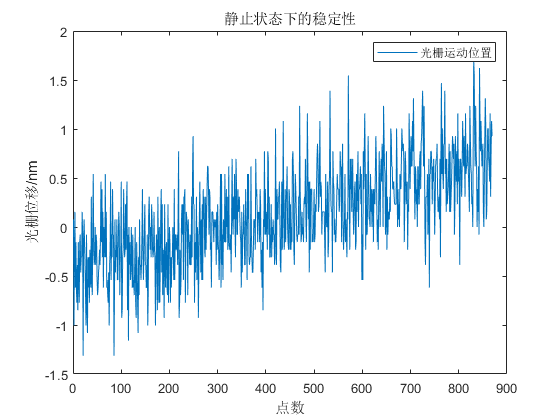
\includegraphics[width=0.8\textwidth]{4-fig//静止状态下的稳定性.png}
  \caption{静止状态下的稳定性}
  \label{fig:静止状态下的稳定性}
\end{figure}

系统稳定性主要受噪声的影响,噪声又可分为低频噪声和高频噪声。本文设计的外差式光栅位移测量系统,外界环境变化的影响可能作为系统的低频噪声,如环境温度变化引起的热漂移,实验装置的振动,此种噪声可以通过改善实验条件来进行减少。高频噪声主要来自于系统的自身元件因素,如激光器的波动等,在实验中是很难进行规避减少的。尽管如此,本课题研究的外差光栅位移测量系统在没有任何补偿的情况下,在测试中仍然表现出良好的稳定性。

\section{误差分析}
\subsection{光栅非理想误差}
本系统采用光栅栅距作为测量基准,而不是波长,因此对于光栅的要求会比光源更高。在制造过程中,光栅的最终质量会因制造工艺或使用的材料而受到影响。光栅的质量会影响光栅的参数,如光栅栅距的大小和均匀性,以及狭缝的宽度。

光栅的刻划误差主要可分为周期刻划误差和累积刻划误差。
\subsubsection{周期误差分析}

在光栅的制造加工过程中,由于各种因素的影响,任意两条光栅线之间的距离并不完全相等,光栅栅距会周期性的变化,这种情况产生的误差就是周期性误差。当光栅的光栅栅距在激光束内发生变化时,称为短周期划线误差;当光栅的光栅栅距在激光束外发生变化时,称为中长周期划线误差。本文使用的光栅线密度为1200线/mm,光栅栅距为833nm,入射光束光斑直径为3mm,包括多条光栅线,光电探测器接收一定区域内的光强信息,得到干涉条纹是大量光栅线共同工作的平均结果,由于在位移测量中需要扫过大量栅线,各个栅线的距离被平均效应所削弱,因此短周期刻划误差的影响大大衰减。

假设实际参与衍射作用的光栅栅线数为n,单个栅线的位置偏差为$\sigma_{0}$,则最终产生的干涉条纹位置标准差$\sigma$为:
\begin{equation}
  \sigma=\frac{\sigma_{0}}{\sqrt{n-1}}
\end{equation}

本文所选用的光栅栅距为833nm,光斑直径为3mm,则n=3600。此时:
\begin{equation}
  \sigma=\frac{\sigma_{0}}{60}
\end{equation}
可以看出本文所选用的高线数的光栅的周期刻划误差的数量级在$10^{-2}nm$级,对系统的影响较小。

\subsubsection{累积误差分析}
光栅的累积刻划误差不能通过平均效应进行消除,对测量结果的影响较大。

在第二章的多普勒频移分析中我们知道,当光栅运动时,两束光的多普勒频差为:
\begin{equation}
  \Delta f=2 \frac{v}{D}
\end{equation}

假设光栅入射位置的累积误差为$\Delta D$,则多普勒频差变为:
\begin{equation}
  \Delta f^{\prime}=2 \frac{v}{D+\Delta D}
\end{equation}

从而引起的相位偏差为:
\begin{equation}
  \Delta \varphi=2 \pi \int_{0}^{t}\left(\Delta f-\Delta f^{\prime}\right) d t=4 \pi S\left(\frac{1}{D}-\frac{1}{D+\Delta D}\right)=4 \pi S \frac{\Delta D}{D(D+\Delta D)}
\end{equation}

由于$\Delta D \ll D$,故上式可写为:
\begin{equation}
  \Delta \varphi=4 \pi S \frac{\Delta D}{D^{2}}
\end{equation}

光栅的相位差和栅距误差成正比,由于相位差所引起的干涉条纹移动量可表示为:
\begin{equation}
  \Delta S=2S \frac{\Delta D}{D^{2}}
\end{equation}

由上式可以看出,当光栅沿着运动方向位移S后,光栅栅距的误差会随着位移的长度进行线性累积。假设光栅移动1mm,光栅栅距的累积误差为50nm,引起相应的测量误差会达到144nm,因此累积误差时对测量结果影响比较大的误差源,且这个误差源在整个测量过程中的分布又是不均匀的,如果能有光栅的误差数据,可以对累积误差项进行补偿。这一部分将会放在第五章进行讨论和实验。

\subsection{几何误差}
\subsubsection{光栅安装误差}
理想安装情况下,光栅的法线方向应与运动台的运动方向保持垂直,在这种情况下,测得的光栅位移就是运动台的位移。但是考虑到在安装过程中可能存在的误差,光栅的固定位置与移动方向之间总是存在一定的偏角,导致测量结果的不准确。

为了清晰描述光栅与运动台之间的位置关系,建立如图\ref{fig:光栅安装误差}所示坐标系。主要从绕X、Y、Z轴偏转和沿X、Z两个轴偏移等五个量来考虑光栅与理论移动方向的偏转误差。
\begin{figure}[H]
  \centering
  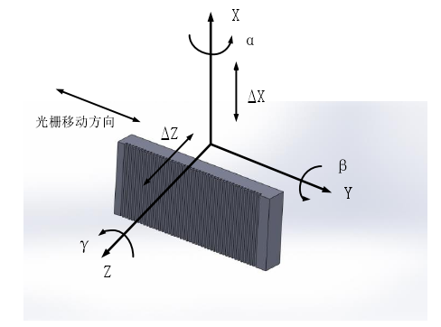
\includegraphics[width=0.7\textwidth]{4-fig//光栅安装误差.png}
  \caption{光栅安装误差}
  \label{fig:光栅安装误差}
\end{figure}

借助于齐次变换矩阵,可以将光栅上某点的理想坐标(x,y,z)转换为实际坐标(X,Y,Z),两者通过一定的坐标转换关系得到。
\begin{equation}
  \begin{aligned}
    \left[\begin{array}{l}
        X \\
        Y \\
        Z
      \end{array}\right]
     & =\left[\begin{array}{ccc}
        \cos \gamma & -\sin \gamma & 0 \\
        \sin \gamma & \cos \gamma  & 0 \\
        0           & 0            & 1
      \end{array}\right]\left[\begin{array}{ccc}
        \cos \beta  & 0 & \sin \beta \\
        0           & 1 & 0          \\
        -\sin \beta & 0 & \cos \beta
      \end{array}\right]\left[\begin{array}{ccc}
        1 & 0           & 0            \\
        0 & \cos \alpha & -\sin \alpha \\
        0 & \sin \alpha & \cos \alpha
      \end{array}\right]\left[\begin{array}{l}
        x \\
        y \\
        z
      \end{array}\right] \\
     & =\left[\begin{array}{cccc}
        \cos \gamma \cos \beta & -\sin \gamma \cos \alpha+\cos \gamma \sin \beta \sin \alpha & \sin \gamma \sin \alpha+\cos \gamma \sin \beta \cos \alpha  \\
        \sin \gamma \cos \beta & \cos \gamma \cos \alpha+\sin \gamma \sin \beta \sin \alpha  & -\cos \gamma \sin \alpha+\sin \gamma \sin \beta \cos \alpha \\
        -\sin \beta            & \cos \beta \sin \alpha                                      & \cos \beta \cos \alpha
      \end{array}\right]\left[\begin{array}{l}
        x \\
        y \\
        z
      \end{array}\right]
  \end{aligned}
\end{equation}

光栅沿Y轴方向移动,当理论位移为$y$时,由矩阵转换关系可以得到光栅实际位移为
\begin{equation}
  y^{\prime}=(\cos \alpha \cos \gamma-\sin \alpha \sin \beta \sin \gamma) y
\end{equation}
测量误差$\Delta y$为:
\begin{equation}
  \Delta y=y^{\prime}-y=(\cos \alpha \cos \gamma-\sin \alpha \sin \beta \sin \gamma-1) y
\end{equation}
实际测量中$\alpha $,$\beta $,$\gamma $可以理解为一个固定的角度,是一个常数,则测量误差$\Delta y$为与实际位移量$y$成线性相关关系。

在1°误差角,100um的行程下,由于光栅偏转安装所引起的误差为-31.13nm

\subsubsection{读数头安装误差}
将光栅与运动台固定好后,需要对读数头进行安装。理想安装情况下,光束有光纤射入读数头内部的反射镜,垂直入射到光栅表面,随后在二次衍射后垂直于光栅射出,而在实际中,由于装配的问题,读数头相对于光栅表面会存在一定偏角,使得测量结果出现误差。

为了清晰描述光栅和读数头之间的位置关系,以光栅的位置作为固定坐标系,读数头相对于光栅的安装位置就可以用坐标系来进行描述。可以将读数头的误差划分为横滚、俯仰和偏航三种情况。

(1)读数头横滚误差

当读数头相对于理想位置出现横滚时,读数头出射的光以一定的角度$\alpha $倾斜射入光栅,但光束仍然在光栅的法线平面内,将出射光分为两部分,$cos \alpha $部分正常垂直入射到光栅,$sin\alpha $部分离开光栅。这种偏转同样不会影响到测量结果,但是减弱了光的强度,可能导致测量光光强不够,光电转换信号不行。在调试过程中,可以用光强计测量出射光的强弱变化来调节角度。

读数头存在横滚误差的示意图如图\ref{fig:读数头横滚误差三视图}所示。
\begin{figure}[H]
  \centering
  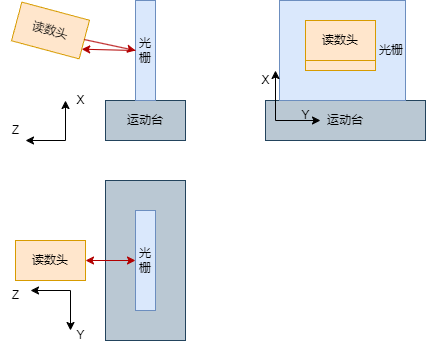
\includegraphics[width=0.7\textwidth]{4-fig//读数头横滚误差.png}
  \caption{读数头横滚误差}
  \label{fig:读数头横滚误差三视图}
\end{figure}

(2)读数头俯仰误差

当读数头相对于理想位置出现俯仰时,会改变入射光的入射角,从而导致第一次衍射的±1级衍射光不再一样的角度射入角锥棱镜,经角锥棱镜返回的光束在光栅上发生二次衍射后的二级衍射光不能垂直返回读数头,携带的位移信息不再准确。

读数头存在横滚误差的示意图如图\ref{fig:读数头俯仰误差三视图}所示。

(3)读数头偏航误差

当读头相对于理想位置存在偏航误差角时,系统不会产生测量误差,仍能准确测量一维光栅的位移变化。但是在实际装配过程中,如果存在偏航误差,两束光束不能准确汇合,通过调试能够避免此问题,在组装阶段就发现问题,因此在实际位移测量中不会出现偏航误差。

读数头存在横滚误差的示意图如图\ref{fig:读数头偏航误差三视图}所示。

\begin{figure}[H]
  \centering
  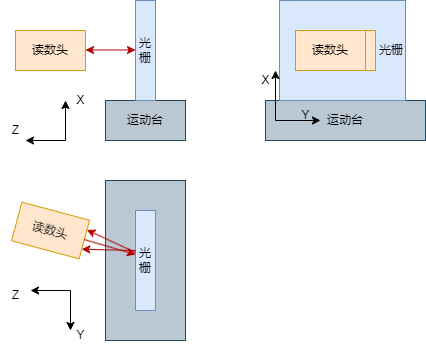
\includegraphics[width=0.7\textwidth]{4-fig//读数头俯仰误差.png}
  \caption{读数头俯仰误差}
  \label{fig:读数头俯仰误差三视图}
\end{figure}
\begin{figure}[H]
  \centering
  \includegraphics[width=0.7\textwidth]{4-fig//读数头偏航误差.png}
  \caption{读数头偏航误差}
  \label{fig:读数头偏航误差三视图}
\end{figure}



\subsection{测量环境误差}
作为一种干涉测量法,相比于激光干涉仪,光栅位移测量系统对测量环境要求比较宽松,但是外界振动、温度变化、空气扰动等影响对测量系统的精度仍然有一定影响。例如振动会引起干涉条纹振荡,温度变化会影响光栅栅距,空气扰动会使得干涉条纹产生偏移。本系统采用对称式光路设计,尽可能减少环境对其产生的影响。

(1)温度影响

由于光栅位移测量系统是以光栅栅距作为测量基准的,温度变化会引起栅距变形,甚至会影响光栅表面形状,对测量结果产生影响。设光栅的指定工作温度为$t_{0}$,实际工作温度为$t$,此时光栅栅距和光栅长度与温度变化的关系如下:
\begin{equation}
  \frac{\Delta d}{d}=a\left(t-t_{0}\right) \quad \frac{\Delta L}{L}=a\left(t-t_{0}\right)
\end{equation}
其中a代表光栅的线膨胀系数。本测量系统光栅所使用的光栅基地为K9玻璃,其膨胀系数为$\mathrm{a}=7.6 \times 10^{-6} \mathrm{~K}^{-1}$,光栅的长度为25mm,光栅栅距为833nm,当温度变化1°时:
\begin{equation}
  \Delta d=833 \times 7.6 \times 10^{-6} \mathrm{~nm}=0.0063 \mathrm{~nm}
\end{equation}
\begin{equation}
  \Delta L=25 \times 7.6 \times 10^{-6} \mathrm{~mm}=190 \mathrm{~nm}
\end{equation}

从上式可以看出,温度对于栅距的影响极小,但是对于光栅的整体尺寸的影响不容忽视。对于温度引起的误差,在精密位移测量系统中,通常会实时测定光栅的环境温度,通过软件进行补偿来提高精度。但是由于材料的本身问题及温度测量过程中也可能出现误差,所以这种温度补偿的精度不会太高。本实验在测量过程中控制环境温度为恒定,并将测量系统用密闭空间进行封闭,以尽可能减少温度对其的影响。

(2)振动及空气扰动的影响

对于光栅测量系统来说,振动是影响测量精度的主要误差源,因此在测量环境中要避免大的振动。对测量系统振动的影响主要包括两部分:一是外界环境引起整个系统的振动。如果读数头和光栅导轨振动的振幅和频率相同,则读数头和光栅导轨相对静止,基本上对测量精度没有影响;另一种是光栅导轨运动引起的单一振动,如导轨的直线度和运动速度不均匀。这种振动包含很多频率成分,通过滤波可以滤除一部分。由于本系统采用对称光路结构,空气扰动对测量精度的影响可以忽略。

由于振动引起的测量误差很难用数据来描述,而且会造成很大的计数误差,所以在工作环境中,要尽量选择较好的环境,或者采取减震、抗干扰等措施来避免这种误差。

综上所述,在光栅位移测量系统中,温度误差对光栅尺寸的变化影响很大,因此在测量过程中要保证恒温。振动和空气扰动只能通过合理设计系统结构和隔离较好的测量环境来解决。

\section{非共光程光路误差}
对于传统的干涉位移测量方法,所设计的光路结构中,参考光路和测量光路存在非共光程光路,在实际测量过程中,其测量精度和稳定性受环境影响因素限制。本文所设计的光路结构也存在类似情况,同样会受到环境中空气折射率的影响。

\subsection{空气折射率计算方法}
对于光栅位移测量系统,空气折射率的变化会影响到非共光程光路的光程变化,进而引起测量误差。为了保证测量的精度,不影响到最后测量结果的准确性,在实验测量过程中需要对空气折射率进行实时测量和补偿。测量空气折射率的方法主要分为直接测量法和间接测量法。直接测量法\cite{李东光2000真空腔测量空气折射率的方法及精度分析,minoshima2011high,fang2002heterodyne}是将激光分别穿过相同光程差距离的空气腔和真空腔,计算所对应得距离和腔长直接得到空气折射率,该测量方法精度可达$10^{-8}$,但是实验要求的真空度很高,条件苛刻。实际测量中通常采用间接测量法进行测量,通过温压传感器测量空气中的参数,代入空气折射率计算公式来间接计算空气折射率\cite{yazdani2014application,tualle2003derivation,ferwerda1999radiative},该测量精度能达到$10^{-7}$量级。本文选择使用间接测量法来对实验室的空气折射率进行测量。

使用间接测量法最关键的地方在于空气折射率计算公式是否准确。目前应用最广泛的公式是
1966年由Edlén提出的著名的Edlén经验公式\cite{edlen1966refractive}。随后K. Birch和M. Downs 对Edlén公式进行深入研究,综合考虑大气中二氧化碳含量\cite{birch1988results,birch1993effect,birch1993updated}对空气折射率的影响,于1994年提出了修正的Edlén公式\cite{birch1994correction},其表达式如下:
\begin{equation}
  \left(n_{s}-1\right) \times 10^{8}=8342.54+\frac{2406147}{130-\sigma^{2}}+\frac{15998}{38.9-\sigma^{2}}
  \label{eq:标准干燥空气折射率表达式}
\end{equation}
\begin{equation}
  n_{t p}-1=\frac{p\left(n_{s}-1\right)}{96095.43} \times \frac{1+p(0.601-0.00972 t) \times 10^{-8}}{1+0.0036610 t}
  \label{eq:实际空气折射率表达式}
\end{equation}
\begin{equation}
  n_{t p f}-n_{t p}=-f\left(3.7345-0.001 \sigma^{2}\right) \times 10^{-10}
  \label{eq:潮湿空气折射率表达式}
\end{equation}
其中式\ref{eq:标准干燥空气折射率表达式}是由色散方程推导出的标准干燥空气的折射率表达式,$n_{s}$是标准干燥空气的折射率,无量纲,$\sigma$是真空中的波数,单位为$\mu m^{-1}$。公式\ref{eq:实际空气折射率表达式}是干燥空气在温度t和压力p的折射率表达式,$n_{t p}$是此时空气的折射率,温度t的单位是${ }^{\circ} \mathrm{C}$,压力p的单位是Pa。公式\ref{eq:潮湿空气折射率表达式}是潮湿空气的折射率表达式,$n_{t p f}$是此时空气的折射率,$f$是水蒸气的压强,单位为Pa。

\subsection{实验测试}
为了解光栅位移测量系统的空气折射率变化情况,本文利用温度、压强传感器对实验室内的环境参数进行测量,利用修正后的Edlén公式对空气折射率进行了计算。温度传感器的分辨率为0.00001${ }^{\circ} \mathrm{C}$,压强传感器的分辨率为0.1Pa。

图\ref{fig:温度随时间的变化曲线}为四小时内实验室温度变化情况,从图中可以看出,四小时内实验室环境温度变化范围为0.15${ }^{\circ} \mathrm{C}$。图\ref{fig:压强随时间的变化曲线}为四小时内实验室压强变化情况,从图中可以看出,四小时内实验室压强变化范围为100Pa。默认湿度变化范围为1\%。将测得的环境参数数据代入Edlén公式中,计算得到的空气折射率变化如图\ref{fig:相对折射率随时间的变化曲线}所示。从图中可以看出,实验室在三个小时内的空气折射率波动为$5\times 10^{-7}$,该波动大小与国内其他高标准实验室环境\cite{yan2014measurement}基本处于同一水平。

利用测量得到的实验室空气折射率变化,对光栅位移测量系统的非共光程误差进行研究。根据第三章对于非共光程误差的推导:
\begin{equation}
  \phi_{n o n}=k\left(l_{-1}-l_{+1}\right)
\end{equation}
其中$k=2 \pi n / \lambda$,$n$为空气折射率,$\lambda $为真空中波长。由于本系统采用对称光路结构,$l_{-1}$与$l_{+1}$之间的差值很小。在本文构建的光栅位移测量系统中,经测量两者相差在5mm以内。使用上面测得的空气折射率波动结果,代入上式,由空气折射率变化引起的光栅位移测量系统的非共光程误差约为0.24 nm。

\begin{figure}[htb]
  \centering
  \includegraphics[width=0.8\textwidth]{4-fig//温度随时间的变化曲线.png}
  \caption{温度随时间的变化曲线}
  \label{fig:温度随时间的变化曲线}
\end{figure}

\begin{figure}[H]
  \centering
  \includegraphics[width=0.8\textwidth]{4-fig//压强随时间的变化曲线.png}
  \caption{压强随时间的变化曲线}
  \label{fig:压强随时间的变化曲线}
\end{figure}

\begin{figure}[H]
  \centering
  \includegraphics[width=0.8\textwidth]{4-fig//相对折射率随时间的变化曲线.png}
  \caption{相对折射率随时间的变化曲线}
  \label{fig:相对折射率随时间的变化曲线}
\end{figure}


\section{本章小结}
本章主要介绍了光栅位移测量系统的实验部分,从光路的调试和安装,到实验的性能测试结果。从长行程测试、短行程测试和稳定性测试三个方面对该系统进行评估,实验结果表明本文所设计的光栅位移测量系统具有良好的稳定性和重复性,在行程测试中也能得到良好的测试结果。然后对本系统中存在的误差进行分析,从光栅非理想误差、几何误差、测量环境误差等方面进行分析。最后对非共光程光路误差进行分析,进行空气中折射率测量实验。









\chapter{光栅栅距测量及其误差修正}
\section{栅距误差产生原因}
衍射光栅的制造方法主要分为机械刻划法和光刻法。其中,机械刻划法是指用光栅机械刻划机对光栅进行刻划,在实际制造过程中是使用金刚石刀具在光栅基底的膜层上通过机械运动刻划出一系列具有一定形状的沟槽阵列。光栅刻划的过程如图\ref{fig:光栅刻划过程}所示。
\begin{figure}[H]
  \centering
  \includegraphics[width=9cm]{5-fig//光栅刻划过程.png}
  \caption{光栅刻划过程}
  \label{fig:光栅刻划过程}
\end{figure}

光刻法制作光栅的过程主要分为涂胶、光刻、刻蚀、清洗四个步骤。

涂胶是光刻前要做的准备工作。其工艺是先将基板清洗干燥,然后将光刻胶均匀地涂在基板上。

在光刻过程中,先在基板上涂上一层光刻胶后,通常借助具有图案结构的掩模版进行曝光,然后将基材浸泡在显影液中,这样曝光的地方就会被溶解,至此在光刻胶上制作了所需的结构。常用的光刻方法主要有电子束光刻和全息光刻。电子束光刻利用电子形成光束,将其聚焦到一个非常小的点,形成纳米级光斑,直接在光刻胶上书写所需的结构;全息光刻利用两束光的干涉条纹对光刻胶基板进行直接曝光,并将干涉条纹的周期信号记录到光刻胶中,从而形成光栅。

刻蚀是通过物理或化学方法去除基板上不需要的部分的过程。在进行过光刻之后,我们需要将光刻结构进行保存,以便重复利用,此时我们就需要使用刻蚀方法将光刻胶上的结构复制转移到能够进行重复利用的基板上。刻蚀方法通常分为两种,一种是干法刻蚀,另一种是湿法刻蚀。干法蚀刻是指先将能与基板发生化学反应的气体转化为等离子体,然后利用等离子体对基板进行蚀刻。这样,没有光刻胶的地方会被等离子体直接轰击,刻蚀出凹槽。湿法蚀刻是指将涂有光刻胶的基板直接浸入能与基板发生反应的溶液中,使基板上有光刻胶的地方受到保护,没有光刻胶的地方会被溶液腐蚀,刻蚀出沟槽。

清洗后,刻蚀完成后,光刻胶就失去了作用。此时,用不与基板反应的溶液清洗光刻胶。最后,将所需的光栅结构留在基板上。

无论采用哪种制造方法,光栅都可能因加工误差而变得不准确。光栅线误差可分为三个方面:单周期误差、光栅的累积误差和刻线清晰度。

单周期误差是指相邻两条光栅线之间的距离与标准光栅常数之差,具体表现为两刻线之间的距离过大或过小。一般来说,单周期误差是在光栅的制造过程中,由于加工机床或工具的随机振动引起的。

光栅的累积误差是指平均光栅间距与标准光栅常数在较大范围内的差值。一般来说,累积误差是在光栅的制造过程中,由于加工机床的长周期误差或者环境中的温度变化等因素引起的。由于光栅位移测量是以光栅间距为测量基准,光栅间距的累积误差将直接反映在测量结果中,而位移测量误差与光栅的累积误差呈线性关系,测量误差随着测量范围的增加而呈线性增加。因此,在测量过程中应尽量避免,并且应采取一定补偿方法对其进行修正。

刻线清晰度是指光栅栅线边缘的清晰平整程度。在加工过程中,由于刻蚀工具等问题,光栅栅线的边缘可能会出现毛刺情况。在光栅位移测量系统中,刻线清晰度不会影响到测量结果,但是会影响到衍射光束的质量,从而影响到最后叠加干涉条纹的清晰程度,增加了辨识的难度。

光栅栅距是光栅位移测量的基准,其精度与最后位移测量系统的精度息息相关。一般光栅会给出标准光栅栅距的大小,但不会给出每个光栅栅距的精确数值。在实际测量过程中,通常认为光栅在各个位置的光栅栅距都为一定值,在测量精度较低、测量范围较小时,光栅栅距的误差影响不大,可以忽略不计。但是在进行纳米级位移测量时,光栅栅距的不均匀就会影响到测量结果,此时就需要对每个光栅栅距进行精确测量和校正,减少累积误差。

\section{光栅栅距测量}
\subsection{光栅栅距测量原理}
本文根据激光干涉原理和光栅衍射原理,基于对比和标定原理提出了测量光栅栅距的新方法。整个光栅栅距测量的工作流程为:首先,将光栅和反射镜固定在运动台上,搭建干涉仪位移测量系统和光栅位移测量系统;然后启动运动台,同时记录干涉仪运动位移和光栅实际位移,在计算机中显示;在matlab中对数据进行处理,通过干涉仪运动位移计算理论经过栅线条纹数,通过光栅实际位移计算这一段的实际栅距平均值,输出光栅栅距及其均匀性。

\subsection{光栅栅距测量方案设计}
光栅栅距对比测量主要基于激光干涉原理和光栅衍射原理,在光栅运动过程中将光栅栅距转换为干涉仪和光栅位移对比量。如图\ref{fig:光栅栅距测量原理图},初始化光栅和干涉仪测量系统,使用控制软件操作超精密运动台以步距$ h $进行连续位移运动,光栅和反射镜附着在运动台上一起运动。在每一个步距$ h $内,记录激光干涉仪的位移测量结果$ L_{i} $,光栅位移测量结果$ S_{i} $,通过记录的数据计算每一个步距$ h $对应的光栅理论位移 $ L=L_{i+1} - L{i} $ 和实际位移$ S=S_{i+1} - S{i} $。

计算每一个步距对应的平均栅距\( p=\frac{S}{L/ D} \),其中光栅理论栅距为 $ D $,激光波长为$ \lambda $。由各个位置的平均栅距计算均方差得到栅距均匀性。
重复测量,得到多组均方差,采用多组均方差的平均值作为光栅栅距均匀性的衡量标准。
\begin{equation}
  \sigma=\sqrt{\frac{\sum_{i=1}^{n}\left(p_{i}-\bar{p}\right)^{2}}{n-1}}
\end{equation}

\begin{figure}[H]
  \centering
  \includegraphics[width=0.5\textwidth]{5-fig/栅距测量流程图.png}
  \caption{栅距测量流程图}
  \label{fig:栅距测量流程图}
\end{figure}

\begin{figure}[H]
  \centering
  \includegraphics[width=1\textwidth]{5-fig/光栅栅距测量原理图.png}
  \caption{光栅栅距测量原理图}
  \label{fig:光栅栅距测量原理图}
\end{figure}


\subsection{双频激光干涉仪位移测量}
双频激光干涉仪是在单频激光干涉仪的基础上结合外差干涉技术研制而成,其光路结构如图\ref{fig:双频激光干涉仪原理图}所示。

当 He-Ne 激光器加上轴向磁场时,由于塞曼效应,激光器会发出左旋和右旋两种不同频率的圆偏振光。圆偏振光通过四分之一波片后形成两个频率为$f_{1}$和$f_{2}$的偏振方向互相垂直的线偏振光。经过分光镜1后,透射光垂直入射到偏振分光镜2上,按照偏振状态不同被分成两束。频率为$f_{2}$的光穿过偏振分光棱镜后射向可移动的三角棱镜4上,当动镜4以速度$\upsilon $运动时,由于多普勒效应,反射回来的光的频率变为$f_{2} \pm \Delta f$(正负号取决于运动方向),频率为$f_{1}$的光反射到固定的角锥棱镜3,反射回的光束与射向动镜的光束重叠,作为系统的测量信号,输出至光电探测器中,此时接收到的频率为$f_{1}-\left(f_{2} \pm \Delta f\right)$。在分光镜1处反射的光作为参考信号由光电探测器接收,此时接收到的频率为$\Delta f = f_{1}-f_{2}$。参考信号和测量信号一同送入板卡中进行处理得到多普勒频移$\Delta f$,通过后续的数据处理得到位移信息。
\begin{figure}[H]
  \centering
  \includegraphics[width=1\textwidth]{5-fig/双频激光干涉仪.png}
  \caption{双频激光干涉仪}
  \label{fig:双频激光干涉仪原理图}
\end{figure}
若测量动镜移动速度为$ \upsilon $,则两路信号的多普勒频差$\Delta f$为:
\begin{equation}
  \Delta f=\frac{2 v}{c} f=\frac{2 v}{\lambda}
\end{equation}
位移测量的距离L可表示成:
\begin{equation}
  L=\int_{0}^{t} v \mathrm{~d} t=\int_{0}^{t} \frac{\Delta f \lambda}{2} \mathrm{~d} t=\frac{\lambda}{2} \int_{0}^{t} \Delta f \mathrm{~d} t \frac{1}{2}=N \frac{\lambda}{2}
\end{equation}
其中$\lambda$表示实际测量时激光的波长值,N为干涉的条纹数。

采用双频激光干涉仪来进行位移测量,最后得到的信号为一交流信号,当被测物体静止时,双频激光干涉仪仍能输出一个固定的交流信号,当被测物体运动时,信号的频率会在静止时的信号频率上增加或减少。与单频激光干涉仪相比,双频激光干涉仪受外界环境干扰因素影响较小,适用于生产现场的测量,并且可以进行远距离测量。

本文设计的激光干涉测量系统如图\ref{fig:测量光路}和\ref{fig:参考光路}所示,光源模块发射出的线偏振光垂直入射到偏振分光镜PBS上,按照偏振状态不同被分成两束,其中频率为$f_{1}$的光反射到固定的角锥棱镜,经过两次四分之一波片从出口射出,作为系统的参考光。频率为$f_{2}$的光穿过PBS后射入可移动的测量动镜,当反射镜以速度$\upsilon $运动时,由于多普勒效应,反射回的光频率变成$f_{2} \pm \Delta f$(正负号取决于运动方向),作为系统的测量信号。随后穿过偏振分光镜后与角锥棱镜反射回的参考光束重叠,得到含有测量距离信息拍频信号$f_{1}-\left(f_{2} \pm \Delta f\right)$,耦合进光纤,由板卡从多普勒频移$\Delta f$调节出干涉条纹的变化数目N即可得到被测物体的位移。
\begin{figure}[H]
  \centering
  \includegraphics[width=8cm]{5-fig/测量光路.png}
  \caption{测量光路}
  \label{fig:测量光路}
\end{figure}
\begin{figure}[H]
  \centering
  \includegraphics[width=8cm]{5-fig/参考光路.png}
  \caption{参考光路}
  \label{fig:参考光路}
\end{figure}
此干涉仪利用四分之一波片对光束的偏振状态进行转换,使光束往返两次通过测量镜,基础分辨力为$\lambda /4$,激光波长$\lambda$为633nm,带入计算可得分辨力约 0.16μm。同时使用三轴激光外差信号解调器对信号进行细分。采样点数为200,并进行2048倍的电子细分,细分后分辨力达到0.3nm。
\begin{figure}[H]
  \centering
  \includegraphics[width=5cm]{5-fig/干涉仪实物图.jpg}
  \caption{干涉仪实物图}
  \label{fig:干涉仪实物图}
\end{figure}

\section{实验验证}
\subsection{系统搭建}
实现光栅栅距测量的实验装置如图所示,干涉仪位移测量系统位于蓝色虚线内,包括一个单轴平镜干涉仪(PIFM0104T-035),一个He-Ne双频激光器(波长为632.99纳米,光斑直径为6毫米),一个反射镜(M)和一些光纤。光栅位移测量系统位于红色虚线内,包括一个激光模块,一个读数头,一个光栅(G),尺寸为30毫米×10毫米×3毫米,光栅栅距为833纳米(图6),和一些光纤。反射镜和光栅固定在一个超精密运动台(型号)上,反射镜表面和光栅表面互相垂直,运动台运动方向与光栅表面位置平行,当运动台移动时,光栅和干涉仪都可以测得位移。调节反射镜和干涉仪的位置,使干涉仪和反射镜相距60毫米。我们将精密运动台的步距设定为10微米,每运动一个步距停留3秒。为了确保实验方法的准确性,我们通过调整运动步距,停留时间,总行程来进行重复测量,每种变量都会影响到最终的测量结果,选取最优的一组变量进行重复实验得到光栅均匀性。为保证测量的准确性,实验装置设置在一个气浮平台上,并且运动台部分由罩壳包裹,以减少周边环境的影响。
\begin{figure}[H]
  \centering
  \includegraphics[width=1\textwidth]{5-fig/栅距测量实物图.jpg}
  \caption{栅距测量实物图}
  \label{fig:栅距测量实物图}
\end{figure}

\subsection{实验结果}
栅距测量的实验结果如表\ref{table:单个栅距测量实验结果}所示。表\ref{table:单个栅距测量实验结果}中干涉仪的位移作为理论位移,光栅位移测量系统的位移值作为测量位移。通过理论位移计算这段步距经过的理论栅线个数,再计算实际的栅距值。总表中可以看出,5次的测量结果表明单个栅距的测量误差为1.88nm。
\begin{table}[H]
  \centering
  \caption{单个栅距测量实验结果}
  \label{table:单个栅距测量实验结果}
  \begin{tabular}{c|c|c|c|c}
    \hline
    测量次数 & 干涉仪位移 & 光栅位移 & 理论移动栅距个数 & 实际栅距值/nm \\ \hline
    1        & 10055.10   & 10051.24 & 12.06            & 833.65        \\ \hline
    2        & 10072.36   & 10067.16 & 12.08            & 833.76        \\ \hline
    3        & 10060.70   & 10064.23 & 12.07            & 833.04        \\ \hline
    4        & 10049.65   & 10030.45 & 12.04            & 834.92        \\ \hline
    5        & 10040.55   & 10030.69 & 12.04            & 834.15        \\ \hline
  \end{tabular}
\end{table}

随后对整个光栅进行分段,将光栅分为12段,计算每一段的平均栅距,最后计算光栅的均匀性和极差。如表\ref{table:整个光栅栅距测量实验结果}所示,每一段的平均栅距通过计算可以得出,其栅距最大处为834.66纳米,最小处为833.41纳米,最后进行加权平均的标准差为0.34768纳米,极差为1.25436纳米,说明所测量的光栅均匀性较好。
\begin{table}[H]
  \centering
  \caption{整个光栅栅距测量实验结果}
  \label{table:整个光栅栅距测量实验结果}
  \begin{tabular}{c|c|c|c|c|c|c}
    \hline
    \diagbox{分段}{次数} & 1/nm     & 2/nm     & 3/nm     & 4/nm     & 5/nm     & 平均值/nm \\ \hline
    1                    & 833.8421 & 834.8582 & 834.2893 & 834.1131 & 834.0852 & 834.23758 \\ \hline
    2                    & 833.0104 & 833.3020 & 833.6533 & 833.3117 & 833.7928 & 833.41404 \\ \hline
    3                    & 834.7044 & 833.9124 & 834.0776 & 834.0718 & 834.4135 & 834.23594 \\ \hline
    4                    & 833.8886 & 834.8881 & 834.1221 & 834.8646 & 833.4260 & 834.23788 \\ \hline
    5                    & 834.0407 & 833.5122 & 834.3186 & 833.0908 & 833.8122 & 833.7549  \\ \hline
    6                    & 834.7794 & 833.6529 & 833.6956 & 834.6474 & 834.0058 & 834.15622 \\ \hline
    7                    & 834.0014 & 834.4795 & 834.1184 & 834.5945 & 834.3881 & 834.31638 \\ \hline
    8                    & 833.5121 & 833.5003 & 834.4884 & 833.0408 & 834.0497 & 833.71826 \\ \hline
    9                    & 834.8171 & 834.3796 & 834.1932 & 835.0240 & 834.9281 & 834.6684  \\ \hline
    10                   & 833.7639 & 834.7272 & 834.0096 & 833.8078 & 835.0215 & 834.266   \\ \hline
    11                   & 835.1312 & 834.0487 & 834.6026 & 834.7306 & 834.5658 & 834.61578 \\ \hline
    12                   & 834.2746 & 833.9607 & 834.5523 & 834.0543 & 834.5739 & 834.28316 \\ \hline
    标准差               & 0.6163   & 0.5568   & 0.3019   & 0.6894   & 0.4594   & 0.34768   \\ \hline
    极差                 & 2.1208   & 1.5861   & 0.9493   & 1.9831   & 1.5956   & 1.25436   \\ \hline
  \end{tabular}
\end{table}

将本实验结果与基于SEM方法的结果相对比,图\ref{fig:SEM实验结果图}是扫描电子显微镜下光栅的形貌,此方法下测得光栅的标准差为1.145。两种结果对比证明了本文方法的可行性,并且精度相较于传统的直接测量法有了进一步的提升。并且本方法在测量过程中无需多余操作,操作简单方便,与光栅表面无接触,对光栅没有损伤。也可重复用于多个光栅的测量,仅需更换光栅即可开始测量。

\begin{figure}[H]
  \centering
  \includegraphics[width=0.7\textwidth]{5-fig/SEM.eps}
  \caption{SEM实验结果图}
  \label{fig:SEM实验结果图}
\end{figure}

\section{累积误差修正}
\subsection{误差修正方法}
误差分析和修正是每一个项目最后都需要进行的步骤,通过误差修正技术能够显著提高系统的测量精度,并大幅节约成本。目前,对光栅栅距进行误差补偿的方法有两种:一种是逐点补偿,此种方法的补偿精度更高,但也更麻烦,需要提前测量光栅内所有点的具体误差值,然后对正在工作的系统直接进行逐点误差补偿;一种是分区补偿,此种方法的补偿精度稍弱,但所需条件不高。将整个光栅等间隔地划分若干区间,每个区间的误差值需要提前进行测量,当系统正在工作时,会对整个区间来进行补偿。本文仅测量出光栅栅距各个区间的均值,所以采用分区补偿来进行操作。

采用分区补偿法来进行误差修正,需要结合现有的实验数据,通过数学方法建立整个系统的误差模型。首先将有限个采样离散值$(x_{i},\Delta y_{i})$进行存储,再通过数学方法将采样点拟合成一条误差曲线,最后在实际进行测量时就可以利用此曲线进行查找和补。常见的误差拟合曲线方法有插值法和最小二乘拟合法。

\subsubsection{插值法}
插值的过程就是不断逼近的一个过程,具体可以描述为:在区间$[x_0,x_n]$内有n个离散点,各离散点的值$(x_{i},\Delta y_{i})$不相同,且$x_0<x_1<\cdots<x_i<\cdots<x_n (\mathrm{i}=1,2,3 \ldots \mathrm{n})$,求在区间$[x_0,x_n]$内任意一点$x_{i}$的插值$y_{i}$。对于这样一个数学问题,我们可以假设一个连续函数$S(x)$经过所有的离散点,然后就可以构造$f(x)$来逼近$S(x)$,使得$f(x)$也经过所有的离散点,或者离所有离散点的距离最近,这样我们就可以通过$f(x)$来计算区间内任意一点的插值。目前常用的插值方法分为三种,分段线性插值法,多项式插值法和样条插值法。

(1)分段线性插值法

此方法是用已知采样离散点作为拟合直线的两端点,相邻两采样离散点直接用直线进行连接,这样整个系统的误差模型就是一条折线,对于区间内任意一点,都可以用该直线方程求得该点的插值。任意一点的插值计算公式为:
\begin{equation}
  \Delta y_i=\Delta y_{k-1}+\frac{\Delta y_k-\Delta y_{k-1}}{y_k-y_{k-1}}\left[y_i-y_{k-1}\right]
\end{equation}

其中$k-1<i<k $。

分段线性插值法计算方法简单,运算量不大,但是在已知离散点附近的曲线并不平滑,可能存在较大的拟合误差,因此在高精度误差补偿场合大多不采用此种方法。

(2)多项式插值法

多项式插值法在分段线性插值法的基础上更进一步,将两点之间的曲线拟合为一个高阶多项式,再用插值的方法求得需要修正的误差值。根据插值多项式的唯一性可知,通过给定的n个离散点可以唯一的做一条n次曲线$f(x)$作为拟合曲线。多项式插值有很多种形式,其中最具有代表性的方法是拉格朗日插值和牛顿插值法。两种方法输出的多项式形式基本一样,只不过表示的形式不同。

对于节点$\left(x_k, \Delta y_k\right)(\mathrm{k}=0,1,2, \ldots, \mathrm{n})$ 拉格朗日插值法,其构造形式为:
\begin{equation}
  \Delta y=f_n(x)=\sum_{k=0}^n\left(\Delta y_k \prod_{j=0, j \neq k}^n \frac{x-x_j}{x_k-x_j}\right) \quad(\mathrm{k}=0,1,2, \ldots, \mathrm{n})
\end{equation}

将插值点$x_i$代入上式,即可求得插值误差$\Delta y$为:
\begin{equation}
  \Delta y_i=\sum_{k=0}^n\left(\Delta y_k \prod_{j=0, j \neq k}^n \frac{x_i-x_j}{x_k-x_j}\right) \text {, 其中 } x_0<x_i<x_n
\end{equation}

拉格朗日插值法插值结构紧凑,一般适用于插值点较少的情况,当插值点数增加时,由拉格朗日插值法构造的插值函数的阶次也就增加了,在拟合曲线上的表现就是严重的震荡现象,这也影响到最后补偿的效果。

(3)样条插值法

样条插值法相较于多项式插值法解决了高阶多项式震荡问题,同时比分段线性插值法曲线更为光滑,拟合效果较好。具体来说,样条插值法的构造过程与多项式拟合类似,不同的是样条插值法通过在节点处增加限制保证了其平滑性。现对样条插值法中的三次样条拟合做介绍:

首先介绍满足三次样条插值函数的定义:

1.三次样条曲线在衔接点处是连续光滑

2.三次样条的一阶导数和二阶导数是连续的

3.每一个分段都是三次多项式函数曲线

由此可知,对于区间$[x,x_i]$所形成的三次样条曲线$S_i(x)$需满足以下方程:
\begin{equation}
  S_i(x) =a_i+b_i\left(x-x_i\right)+c_i\left(x-x_i\right)^2+d_i\left(x-x_i\right)^3
\end{equation}
\begin{equation}
  S_i^{\prime}(x) =b_i+2 c_i\left(x-x_i\right)+3 d_i\left(x-x_i\right)^2
\end{equation}
\begin{equation}
  S_i^{\prime \prime}(x) =2 c_i+6 d_i\left(x-x_i\right)
\end{equation}

设步长$h_i=x_{i+1}-x_i$,由二阶导连续性$S_i^{\prime \prime}\left(x_{i+1}\right)=S_{i+1}^{\prime \prime}\left(x_{i+1}\right)$可得:
\begin{equation}
  2 c_i+6 h_i d_i=2 c_{i+1}
\end{equation}

设$m_i=S_i^{\prime \prime}\left(x_i\right)=2 c_i$:
\begin{equation}
  d_i=\frac{m_{i+1}-m_i}{6 h_i}
\end{equation}

由$S_i\left(x_{i+1}\right)=y_{i+1}$:
\begin{equation}
  a_i+h_i b_i+h_i^2 c_i+h_i^3 d_i=y_{i+1}
\end{equation}

将a,c,d代入上式可得:
\begin{equation}
  b_i=\frac{y_{i+1}-y_i}{h_i}-\frac{h_i}{2} m_i-\frac{h_i}{6}\left(m_{i+1}-m_i\right)
\end{equation}

由一阶导连续性$S_i^{\prime}\left(x_{i+1}\right)=S_{i+1}^{\prime}\left(x_{i+1}\right)$可知:
\begin{equation}
  b_i+2 h_i c_i+3 h_i^2 d_i=b_{i+1}
\end{equation}

代入所有参数:
\begin{equation}
  h_i m_i+2\left(h_i+h_{i+1}\right) m_{i+1}+h_{i+1} m_{i+2}=6\left[\frac{y_{i+2}-y_{i+1}}{h_{i+1}}-\frac{y_{i+1}-y_i}{h_i}\right]
\end{equation}

得到关于m的n+1阶矩阵方程:
\begin{equation}
  \left[\begin{array}{ccccccc}
      1      & 0                         & 0                         &                           & \cdots                        & 0         \\
      h_{0}  & 2\left(h_{0}+h_{1}\right) & h_{1}                     & 0                         &                               &         & \\
      0      & h_{1}                     & 2\left(h_{1}+h_{2}\right) & h_{2}                     & 0                             &         & \\
      0      & 0                         & h_{2}                     & 2\left(h_{2}+h_{3}\right) & h_{3}                         & \vdots    \\
      \vdots &                           &                           & \ddots                    & \ddots                        & \ddots  & \\
             &                           & 0                         & h_{n-2}                   & 2\left(h_{n-2}+h_{n-1}\right) & h_{n-1}   \\
      0      & \cdots                    &                           & 0                         & 0                             & 1
    \end{array}\right]\left[\begin{array}{c}
      m_{0}  \\
      m_{1}  \\
      m_{2}  \\
      m_{3}  \\
      \vdots \\
      m_{n}
    \end{array}\right]=6\left[\begin{array}{c}
      0                                                             \\
      \frac{y_{2}-y_{1}}{h_{1}}-\frac{y_{1}-y_{0}}{h_{0}}           \\
      \frac{y_{3}-y_{2}}{h_{2}}-\frac{y_{2}-y_{1}}{h_{1}}           \\
      \frac{y_{4}-y_{3}}{h_{3}}-\frac{y_{3}-y_{2}}{h_{2}}           \\
      \vdots                                                        \\
      \frac{y_{n}-y_{n-1}}{h_{n-1}}-\frac{y_{n-1}-y_{n-2}}{h_{n-2}} \\
      0
    \end{array}\right]
\end{equation}

求出所有的m即可得到每段的函数曲线。将$x_i$代入三次样条函数,其中$x_k<x_i<x_{k+1}$,即可得到插值误差$\Delta y_i$。

使用三次样条插值法相比于其他两种插值方法具有函数阶次低,节点处曲线光滑,拟合效果好等优点,在之后的误差补偿中采样此方法来进行对比。

\subsubsection{最小二乘拟合法}
如果在使用误差修正技术之前的实验数据受到干扰,那么此时拟合数据本身就可能不可靠。当某个点的数据严重失真时,就可以采用最小二乘法来进行拟合,相对来说也更为可靠。此方法根据离散点来拟合曲线,这条曲线可以反映误差变化的总体趋势,但不会过所有的离散点。最小二乘法的优点是受单个误差点的影响较小,缺点是可能造成已知点的精度损失。

最小二乘法的基本思想是根据给定离散点$(x_k,\Delta y_k)$找到一个拟合函数$\Delta y_i = f(x_i)$,使得拟合函数的残差平方和最小,残差平方和的计算公式为:
\begin{equation}
  Q=\sum_{k=0}^n\left[\Delta Y_k-f\left(Y_k\right)\right]^2
\end{equation}

\subsection{误差修正实验}
要对光栅位移测量系统进行误差修正,首先需要对光栅测量误差进行定义,所谓测量误差是指测量值和真值之间的差,即$\text { 测量误差 }\left(\Delta Y_k\right)=\text { 测得值 }\left(Y_k\right)-\text { 真值 }\left(L_k\right)$。真值一般是指被测光栅真实位移的值,是一个理想概念,在这里使用激光干涉仪测量位移作为真值,那么由光栅测得的位移真值的估计值就可以由$\text { 被测量真值估计值 }\left(\hat{L}_k\right)=\text { 测得值 }\left(Y_k\right)-\text { 测量误差 }\left(\Delta Y_k\right)$得到。

\begin{figure}[H]
  \centering
  \includegraphics[width=0.8\textwidth]{5-fig//拟合曲线.png}
  \caption{拟合曲线}
  \label{fig:拟合曲线}
\end{figure}

\begin{figure}[H]
  \centering
  \includegraphics[width=0.8\textwidth]{5-fig//误差修正实验结果.png}
  \caption{误差修正实验结果}
  \label{fig:误差修正实验结果}
\end{figure}

根据上文分析的误差修正方法,我们这里采用三次样条插值法,5阶最小二乘法,10阶最小二乘法来进行对比实验。实验行程为2500count,步距为50count,实验环境与栅距测量实验相同。图\ref{fig:拟合曲线}为采用三种方法拟合的曲线。图\ref{fig:误差修正实验结果}为三种方法进行误差修正实验结果。对比三种方法补偿后的误差值可以看出,三次样条在各阶段位移补偿后相较于其他方法误差值明显降低。从图中可以看出光栅位移测量系统在误差修正前为$[-25nm,48nm]$,修正后变为$[-10nm,25nm]$,误差降低了,测量系统的精度得到提升。



\section{本章小结}
本章首先分析了栅距误差产生的原因,将光栅栅距误差分为三种:单周期误差、刻线累积误差和刻线清晰度,重点分析了光栅刻线累积误差。在结合现有的光栅栅距测量方法的基础上,提出了基于激光干涉原理和光栅衍射原理,基于对比和标定原理提出了测量光栅栅距的新方法,在光栅运动过程中将光栅栅距转换为干涉仪和光栅位移对比量。然后进行了实验验证,并将结果与基于SEM的方法进行对比,实验结果表明本文所提出的栅距测量方法具有可行性。最后对累积误差修正方法进行详细介绍,采用三次样条插值法对误差进行修正实验,实验结果表明,在进行误差补偿后,测量精度明显得到提高。




\chapter{总结与展望}
\section{本文工作总结}
半导体技术的不断快速发展也对超精密测量技术提出了新的挑战。在采用光学测量法来进行超精密位移测量的技术中,基于光栅的位移测量系统以光栅栅距作为测量基准,相比于激光干涉仪来说,对于光源的稳频要求不高,且光路结构简单,体积较小,能满足光刻机内部要求,因此本文针对光栅位移测量系统及其光栅栅距测量展开了研究。研究工作中取得了以下成果:

1)设计了一种采用二次衍射光来进行位移测量的光路结构,采用对称式光路设计,减少了环境干扰的影响,提高了光路系统的稳定性。并对系统的光源模块和读数头模块的机械结构进行了重新设计,设计的光源模块能产生本文所需要的外差光源,将读数头模块进行集成化和小型化,能够实现参考信号和测量信号的分离,使之与后续信号解调器的连接更为方便。

2)搭建光栅位移测量系统进行实验。实验从长行程位移测试、短行程位移测试和稳定性测试三个方面对此系统进行评估,结果显示,在行程125$um$的行程下其重复性为3.835$nm$,系统稳定性为$\pm 1nm$,利用激光干涉仪对结果进行比较,决定系数为0.99976,表明实验数据重合度高。实验结果表明本文所设计的光栅位移测量系统能够实现纳米级精度的测量。对光栅位移测量系统进行误差分析。从光栅非理想误差、几何误差、环境误差对系统进行分析。对系统中的非共光程误差进行实验测量,也即对环境因素变化引起的空气折射率变化进行分析。实验结果显示,在实验室环境下,3小时温度变化0.15${ }^{\circ} \mathrm{C}$,压强变化为100$Pa$,计算得到的空气折射率变化在$10^{-7}$量级,由空气中折射率变化引起的非共光程误差约为0.24$nm$。

3)提出了一种新的光栅栅距测量方法。基于激光干涉原理和光栅衍射原理,在运动台运动过程中,将光栅栅距的测量转换为干涉仪和光栅位移对比测量。搭建干涉仪位移测量系统和光栅位移测量系统进行实验,实验结果表明,此方法下各个位置光栅栅距标准差为0.34$nm$,极差为1.2$nm$,能够达到纳米级精度,并与基于扫描电子显微镜的方法结果进行对比,此方法的精度更优于SEM方法,证明了方法的可行性。

4)对光栅位移测量系统的误差进行补偿。本文通过三次样条插值法,对所设计的位移测量系统进行误差补偿,将结果与最小二乘法补偿结果进行对比,实验结果表明,采用的三次样条插值法补偿效果优于最小二乘法,经过误差修正后的测量系统误差从$[-25nm,48nm]$,修正后变为$[-10nm,25nm]$,光栅位移测量系统的精度得到明显提高。


\section{研究工作展望}
1)本文以光刻机内部超精密位移检测作为研究背景,以光栅位移测量系统及其光栅栅距作为研究对象,致力于解决实际工程中的应用难题,所提出的检测系统在实验室内取得了较好的效果,但是由于实验条件有限,未能在实际工程应用中进行实验测试。因此,为了能够更有效的解决实际工程应用问题,后续可以在实际设备中对所设计的检测系统进行验证测试。

2)本文针对光栅栅距的测量提出了新的测量方法,但该方法需要搭建2套系统,应用领域局限于实验室环境,在后续的工作中可以尝试将测量方法改进,减少测量装置体积,简化测量操作,使之得到普遍应用。



% 后置部分包含参考文献、声明页(自动生成)等
\backmatter

% 打印参考文献列表
\printbibliography

\chapter*{简历与科研成果}

\section*{基本信息}

\noindent 邹心愿,男,汉族,1998年11月出生,湖北省荆门市人。

\section*{教育背景}

\noindent 2020年9月--2023年1月 \quad 复旦大学工程与应用技术研究院\quad \quad\quad\quad\quad\quad\quad\quad\quad\quad\quad 硕士

\noindent 2016年9月--2020年6月 \quad 武汉大学动力与机械学院\quad \quad\quad\quad\quad\quad\quad\quad\quad\quad\quad\quad\quad\quad 本科

\section*{攻读工程硕士学位期间完成的学术成果}

\noindent 1. Xinyuan Zou, Zhiping Zhang, Chen Zhang, Xiaofeng Yang. Research on the uniformity of the nano-grating pitch based on comparative measurement. LOPET 2022.






\end{document}